\documentclass[svgnames]{beamer}
\usepackage{animate}
\usepackage{graphicx}
\usepackage{amsmath}
\usepackage{hyperref}
\usepackage{booktabs}
\usepackage{multirow}
\usepackage{changepage}
\usepackage{subfig}
\usepackage{threeparttable}
\usepackage{bbm}
\usepackage{soul}
\usepackage{verbatim}
\usepackage{import}
\usepackage{bibentry}
\ifxetex
  \usepackage{fontspec}
\else
  \usepackage[T1]{fontenc}
  \usepackage[utf8]{inputenc}
  \usepackage{lmodern}
\fi

\newtheorem{proposition}[theorem]{Proposition}

\setbeamercovered{transparent}

\hypersetup{
  colorlinks=true,
  citecolor=blue
}
\usepackage[round]{natbib}
% \usetheme{Singapore}
% \usecolortheme{rose}
\usefonttheme{serif}
\begin{document}

\begin{frame}
\title {An Entrepreneurship Fiscal Multiplier}
\author {Wenlan Luo \\ Georgetown University}
\date{10/9/2015}
\maketitle
\end{frame}

\begin{frame}
\centerline{{\color{blue}Heterogeneity} and {\color{red}Macro Policy}}
\centerline{{Facts} -- {Mechanism} -- {Policy Implications}}
\end{frame}

\begin{frame}{{\color{blue}Heterogeneity} and {\color{red}Macro Policy}}
Facts: {\color{blue} Entrepreneurs} respond differently to {\color{red} Government Spending} compared to other households and firms.
\end{frame}

\begin{frame}{Fiscal multiplier: identified through recursive ordering}
{$(log(G),log(Y),MTR,TB3)$,1947I-2008IV}
\begin{figure}[!ht]
\includegraphics[width=1\textwidth]{../v151001/graph/GYICData.png}
\end{figure}
\end{frame}

\begin{frame}{Entrepreneur fiscal multiplier}
{$(log(G),log(Y),MTR,TB3)$,1947I-2008IV}
\begin{figure}[!ht]
\includegraphics[width=1\textwidth]{../v151001/graph/GIData.png}
\end{figure}
\end{frame}

\begin{frame}{Entrepreneur fiscal multiplier: Ramey's pdvmily shock}
{$(log(G),log(Y),MTR,TB3)$,1947I-2008IV}
\begin{figure}[!ht]
\includegraphics[width=1\textwidth]{../v151001/graph/GIDataRamey.png}
\end{figure}
\end{frame}

\begin{frame}{Mechanism}
\begin{itemize}
\item Government spending is to be financed by tax.
\item ... Tax generates negative income effects, increases labor supply, and decreases saving.
\item ... Wage falls and interest rates rise.
\item ... Entrepreneur sector is more ``labor-intensive''. Profits increase which encourages entry.
\end{itemize}
\end{frame}

\begin{frame}{Mechanism: entrepreneurs use more labor than capital}
{Fractions of factors used in non-corporate sector}
\begin{figure}[!ht]
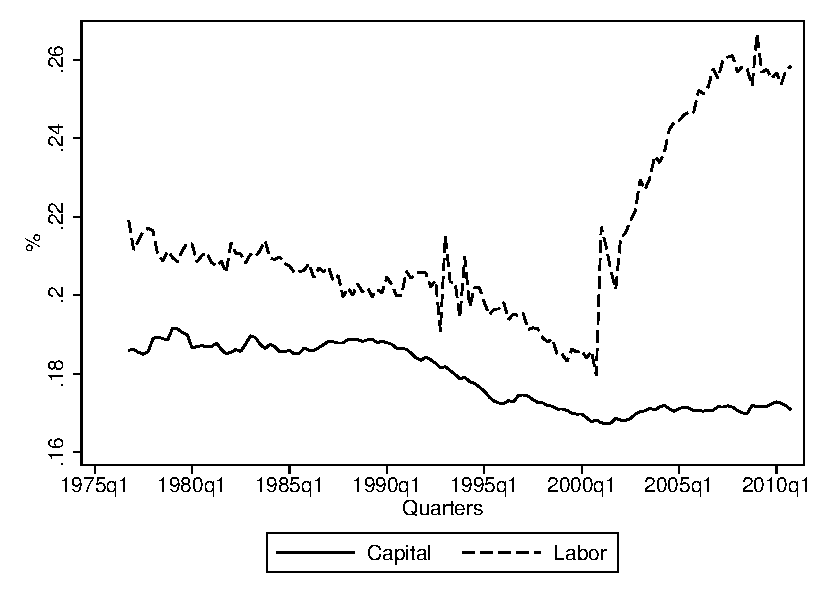
\includegraphics[width=1\textwidth]{graph/klratio.pdf}
\end{figure}
\end{frame}

\begin{frame}{Mechanism}
{Why does entrepreneur sector use more labor than capital?}
\begin{figure}[!ht]
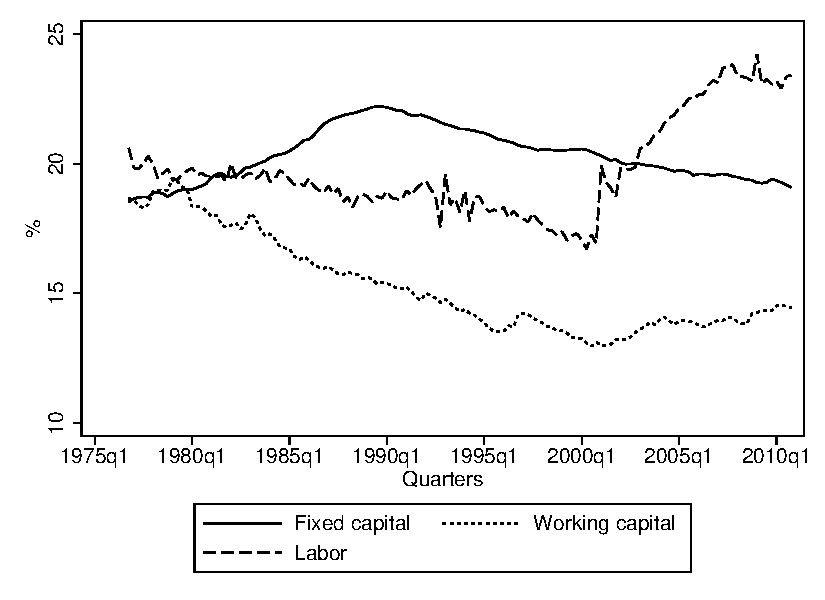
\includegraphics[width=1\textwidth]{graph/wklratio.pdf}
\end{figure}
\end{frame}

\begin{frame}{Mechanism}
{Why does entrepreneur sector use more labor than capital?}
\begin{itemize}
\item It's not (I'm not assuming) different technology...
\item Working capital financing is hampered by financial friction...
\item If this is the case, entrepreneur sector should appear even more ``labor-intensive'' when credit condition is worse...
\item What's in the data?
\end{itemize} 
\end{frame}

\begin{frame}{Mechanism: financial frictions vs labor-intensity}
{Why does entrepreneur sector use more labor than capital?}
\begin{figure}[!ht]
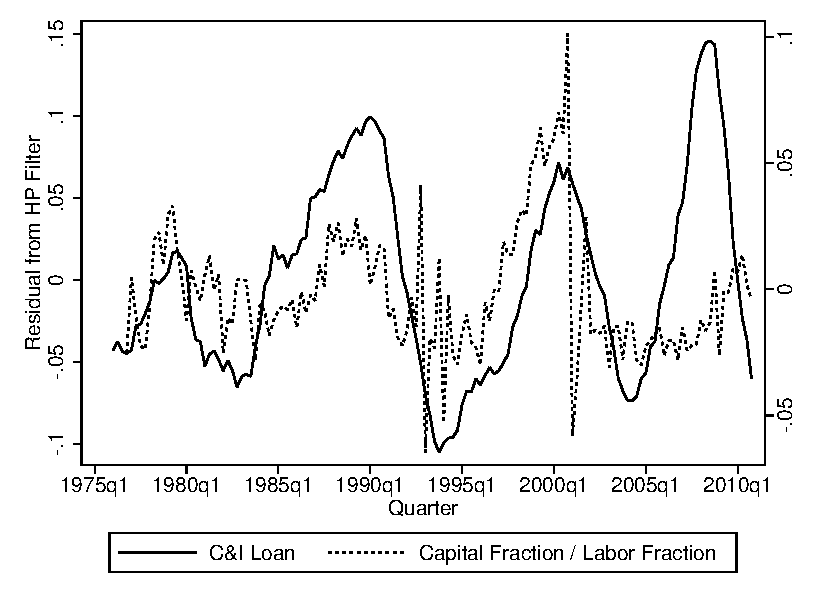
\includegraphics[width=1\textwidth]{graph/loan_klratio.pdf}
\end{figure}
\end{frame}

\begin{frame}{Mechanism}
\begin{itemize}
\item Government spending is to be financed by tax.
\item ... Tax generates negative income effects, increases labor supply, and decreases saving.
\item ... Wage falls and interest rates rise.
\item ... Entrepreneur sector is more ``labor-intensive'' due to financial frictions.
\item ... Profits increase which encourages entry.
\item ... Anticipating profits increase $\Rightarrow$ Marginal productivity of capital increases $\Rightarrow$ Entrepreneurs increase saving (investment) countering the consumption smoothing incentive from negative income effects.
\end{itemize}
\end{frame}

\begin{frame}{Quantitative questions}
Questions:
\begin{itemize}
\item Does this mechanism generate qualitative/quantitative results consistent with data?
\item What are the implications for aggregate response? Does it imply interactions between fiscal policy and other economic conditions?
\end{itemize}
Strategy:
\begin{itemize}
\item A model featuring entrepreneur entry/saving decision which are affected by financial frictions.
\item Calibrated to match (1) fraction of factor use; (2) entrepreneur size distribution; (3) wealth distribution.
\item Feed in government spending shock and inspect the response.
\item Feed in fluctuations of credit conditions and inspect the interactions.
\end{itemize}
\end{frame}

\begin{frame}{Quantitative questions}
Questions:
\begin{itemize}
\item Does this mechanism generate qualitative/quantitative results consistent with data?
\item What are the implications for aggregate response? Does it imply interactions between fiscal policy and other economic conditions?
\end{itemize}
Answers:
\begin{itemize}
\item Model generates responses of entrepreneur entry and investment consistent with data.
\item Generates a sizable output fiscal multiplier close to data, without any Keynesian features.
\item Both entrepreneur and output multipliers are greater when credit is tighter.
\end{itemize}
\end{frame}


\begin{frame}{Related literature}
\begin{itemize}
\item {\color{blue} Mechanism of fiscal multiplier.} \citet{hall_by_2009}, \citet{dyrda_models_2012}, \citet{woodford_simple_2010}, \citet{uhlig_fiscal_2010}.

\item {\color{blue} Distributional effects of fiscal policy.} \citet{heathcote_fiscal_2005}, \citet{bachmann_welfare_2013}.

\item {\color{blue} State-dependent effects of government spending.} \citet{auerbach_measuring_2012}, \citet{owyang_are_2013}, \citet{fazzari_state-dependent_2015}

\item {\color{blue} Entrepreneur entry and saving.} \citet{decker_role_2014}, \citet{quadrini_entrepreneurship_2000}, \citet{cagetti_entrepreneurship_2006}, \citet{buera_financial_2013}.

\item {\color{blue} Heterogeneous agent model with aggregate fluctuations.}
\citet{krusell_income_1997}, \citet{reiter_solving_2009}, \citet{winberry_lumpy_2014}.

\end{itemize}
\end{frame}

\begin{frame}{Model}{Mechanisms and corresponding model elements}
\begin{itemize}
\item Time is discrete. Continuum of Infinitely-lived households with constant measure, a corporate firm, and a government. Single consumption good. Single asset.
\item Households receive shocks on labor productivity and entrepreneur productivity; {\color{blue}choose} to be entrepreneurs and workers; program {\color{blue}consumption/saving}, {\color{blue}labor/leisure}; face tight borrowing constraints across periods.
\item As a worker, household works and receives wages.
\item As an entrepreneur, household does not work; employs capital and labor to produce at market prices.
\item Entrepreneur can finance additional capital within period {\color{blue}up to} a fraction of his own wealth due to financial frictions.
\item A government specifying policies for {\color{blue}bond and tax}.
\item Exogenous government spending shocks, financial shocks, and TFP shocks.
\end{itemize}
\end{frame}

\begin{frame}{Model}{Households' problems: as an entrepreneur}
$$
V^E(\varepsilon,\zeta,a;\Omega) = \max_{k_D,n_D,c,a'}
u(c,l)
+ \beta E V(\varepsilon',\zeta',a';\Omega')
$$
s.t.
$$
\begin{aligned}
c + a' \leq \pi + a - Tax(\Omega) \\
\pi = z \zeta (k_D^{\gamma} n_D^{1-\gamma})^{\theta}
 - r(\Omega)(k_D-a) - \delta k_D - w(\Omega)n_D \\
k_D \leq \lambda a \\
a'\geq 0 \\
l=1\\
\end{aligned}
$$
\end{frame}

\begin{frame}{Model}{Households' problems: as a worker}
$$
V^W(\varepsilon,\zeta,a;\Omega) = \max_{c,l,a'} u(c,l) + \beta E V(\varepsilon',\zeta',a';\Omega')
$$
s.t.
$$
\begin{aligned}
c+a' \leq w(\Omega) \varepsilon(1-l) + a(1+r(\Omega)) - Tax(\Omega) \\
a' \geq 0 \\
0\leq l \leq 1\\
\end{aligned}
$$
\end{frame}

\begin{frame}{Model}{Households' problems: entrepreneur or worker?}
$$
V(\varepsilon,\zeta,a;\Omega) = E_{\tilde{u_E},\tilde{u_W}} \max \{V^E(\varepsilon,\zeta,a;\Omega)+\tilde{u_E},V^W(\varepsilon,\zeta,a;\Omega)+\tilde{u_W}\}
$$
$u_E,u_W$ i.i.d. Gumbel distribution.
$$
V(\varepsilon,\zeta,a;\Omega) = log(exp(V^E(\varepsilon,\zeta,a;\Omega))+exp(V^W(\varepsilon,\zeta,a;\Omega)))
$$
$$
Pr^E(\varepsilon,\zeta,a;\Omega) = \frac{exp(V^E(\varepsilon,\zeta,a;\Omega))}
{exp(V^E(\varepsilon,\zeta,a;\Omega))+exp(V^W(\varepsilon,\zeta,a;\Omega))}
$$
\end{frame}

\begin{frame}{Model}{Closure}
\begin{itemize}
\item Corporate firm:
$$r = z \gamma (\frac{K}{N})^{\gamma-1}, z(1-\gamma) (\frac{K}{N})^{\gamma}$$
\item Government:
\begin{itemize}
\item Promise to pay interest rates of bond equal to interest rate of capital, state by state, following \citet{heathcote_fiscal_2005} and \citet{bachmann_welfare_2013}.
\item Tax rule:
$$
Tax = \rho_0 + \rho_1 B + \rho_2 G
$$
\item Budget:
$$
B'= B(1+r) + G - Tax
$$
\end{itemize}
\item Exogenous process:
$log(z') = \rho_z log(z) + \varepsilon^z$,
$G' = \rho_G G + (1-\rho_G)\bar{G} + \varepsilon^G$,
$\lambda' = \rho_{\lambda} \lambda + (1-\rho_{\lambda})\bar{\lambda}
+\varepsilon^{\lambda}$
\end{itemize}
\end{frame}

\begin{frame}{Model}{Definition of equilibrium}
Individual state $x=(\varepsilon,\zeta,a)$. Aggregate state $\Omega=(z,G,\lambda;B,\Phi)$.
A recursive equilibrium is
\begin{enumerate}
\item Policy and value functions as functions of $(x,\Omega)$: $V(x,\Omega),V^E,V^W,Pr^E,a'^E,a'^W,n,n^D,k^D$
\item Aggregates as functions of $\Omega$: $K(\Omega),N,w,r,Tax$
\item Transition for $B$, $J:\Omega \rightarrow B'$. Transition for $\Phi$, $H: \Omega \rightarrow \Phi'$.
\end{enumerate}
\end{frame}
\begin{frame}{Model}{Definition of equilibrium}
\begin{enumerate}
\item Policy and value functions solve agent's problem.
$$V^{W,E}(x,\Omega) = \max ...
 +\beta EV(\varepsilon',\zeta',a';z',G',\lambda';J(\Omega),H(\Omega))$$
\item Market clear.
$$
\begin{aligned}
& Labor: \int n\cdot (1-Pr^E) d\Phi = \int n^D\cdot Pr^E d\Phi + N \\
& Asset: \int a d\Phi = \int k^D\cdot Pr^E d\Phi + K + B \\
& Interest \ rate: r = z \gamma (\frac{K}{N})^{\gamma-1} \\
& Wage: w = z(1-\gamma) (\frac{K}{N})^{\gamma} \\
\end{aligned}
$$
\item Government policy.
$$
\begin{aligned}
& Tax: Tax=\rho_0 + \rho_1 B + \rho_2 G \\
& Bond: B' = J(B) = B(1+r) + G - Tax
\end{aligned}
$$
\item Transition of $\Phi$ is consistent.
\end{enumerate}
\end{frame}

\begin{frame}{Model solutions}
Challenges:
\begin{itemize}
\item Multiple aggregate shocks and continuous aggregate states. Higher moments matter. De Nardi et al. (2015), \citet{bachmann_welfare_2013}.
\item Pure projection + perturbation (as \citet{reiter_solving_2009}) can't address state-dependent effects.
\end{itemize}
Solutions:
\begin{itemize}
\item Discretize value functions and distributions. Solve non-stochastic steady state.
\item Solve dynamics by linear perturbation around non-stochastic steady state. State variables include the discretized distributions over individual states. Jump variables include the discretized value functions over individual states.
\item Only use linear perturbation as {\bf forecasting rules of future value functions}. In simulations, solve decision problems and market clear conditions exactly, and update future states exactly.
\end{itemize}
\end{frame}

\begin{frame}{Linear forecasting is very accurate}
Forecasting error (\%):
\begin{table}
\begin{tabular}{cccc}
\hline
Vars & 1-step & 100-step & 1000-step \\
\hline
r & 0.4261 & & \\
w & 0.1626 & & \\
$Ea$ & 0.0249 & &  \\
$Ea^2$ & 0.0181 & & \\
$Ea^3$ & 0.0276 & & \\
$Ea^4$ & 0.0382 & & \\
\hline
\hline
\end{tabular}
\end{table}
\end{frame}

\begin{comment}
$$
V(\varepsilon,\zeta,a;\Omega) = log(exp(V^E(\varepsilon,\zeta,a;\Omega))+exp(V^W(\varepsilon,\zeta,a;\Omega)))
$$
$$
Pr^E(\varepsilon,\zeta,a;\Omega) = \frac{exp(V^E(\varepsilon,\zeta,a;\Omega))}
{exp(V^E(\varepsilon,\zeta,a;\Omega))+exp(V^W(\varepsilon,\zeta,a;\Omega))}
$$
\end{comment}

\begin{frame}{Calibration}{Parameters fixed exogenously}
$u=\frac{(c^{\chi}l^{1-\chi})^{1-\sigma}}{1-\sigma}$, $\sigma=2$

$F(K,L) = zK^{\gamma}L^{1-\gamma}$, $\gamma=0.36$

$\varepsilon$, $\varepsilon'=\rho_{\varepsilon}\varepsilon + e'$, $\rho_{\varepsilon}=0.94$,$\sigma^2_{\varepsilon}=0.01$

$z$, $\rho_z=0.75$, $\sigma_z=0.012$, US Data

$G$, $\rho_G=0.8909$, $\sigma_G=0.0145\bar{G}$, US Data

$\lambda$, $\rho_{\lambda}=0.9170$, $\sigma_{\lambda}=0.049$, matching anecdotal evidence (Khan and Thomas (2013)):
\begin{quote}
...debts falling more than $26\%$ as a financial crisis...
...13 crises in the last 200 years (800 quarters)...
...Average duration is 2 years...
\end{quote}
\end{frame}

\begin{frame}{Calibration}{Parameters calibrated to match moments}
\begin{table}[htbp]
  \centering
    \begin{tabular}{ccccc}
    \toprule
    Parameters & Value & Target & Data  & Model \\
    \midrule
    $\delta$ & 0.021 & r     & 0.0125 & 0.0125 \\
    $\beta$ & 0.980 & K/Y &  10.6 & 10.85 \\
    $\chi$ & 0.31  & $\bar{n_w}$ & 0.33  & 0.33 \\
    \midrule
    $p_1$ & 0.0039  & \% Entrepreneurs & 0.0755  & 0.072 \\
    $p_2$ & 0.97 & Gini & 0.81 & 0.76 \\
    $\mu_{\zeta}$ & 0.76    & \% Size 1-5 & 0.7510 & 0.7768 \\
    $\sigma_{\zeta}$ & 0.23 & \% Size 6-10 & 0.1460 & 0.1124 \\
    \midrule
    $\theta$ & 0.76 & Capital fraction & 0.1780 & 0.1854 \\
    $\lambda$ & 1.32 & Labor fraction & 0.2180  & 0.2086 \\
    \midrule
    $\bar{Tax}$ & 1.68 & G/Y & 0.2086 & 0.2086 \\
    $\bar{B}$ & 0.3597 & B/Y & 1.2 & 1.2 \\
    \bottomrule
    \end{tabular}%
  \label{tab:addlabel}%
\end{table}%
\end{frame}

\begin{frame}{Model performance}{Size and wealth distribution}
Size of entrepreneur firms measured by employment level, KFS
\begin{table}[htbp]
  \centering
  
    \begin{tabular}{cccccc}
    \toprule
    & 1-4 & 5-9 & 10-19 & 20-99 & 100+ \\
    Data & 75.1 & 14.6 &  6.6  & 3.5  & 0.3 \\
    Model & 77.7 & 12.4 & 5.0 & 4.9 & 0.0 \\
    \bottomrule
    \end{tabular}%
    
\end{table}
Wealth distribution, SCF, \citet{diaz-gimenez_facts_2011}
\begin{table}[htbp]
  \centering
  
    \begin{tabular}{cccccc}
    \toprule
    & Top 1\% & Top 5\% & Top 10\% & Top 20\% & Gini\\
    Data & 30 & 51 & 64 & 79 & 0.79 \\
Model & 23.8 & 57.6 & 82.5 & 91.2 & 0.76 \\
\bottomrule
    \end{tabular}%
\end{table}

TODO(wenlan): business cycle property
\end{frame}

\begin{frame}{Roadmap for results}
\begin{itemize}
\item Entrepreneur fiscal multiplier.
\item Implied for output.
\item State-dependent effects.
\end{itemize}
\end{frame}

\begin{frame}{Entrepreneur fiscal multiplier}
{Response to +G shock at period 1}
\begin{figure}[!ht]
\includegraphics[width=1\textwidth]{../v151001/graph/GIModel.png}
\end{figure}
\end{frame}

\begin{frame}{Entrepreneur fiscal multiplier}
{Response to +G shock at period 1}
\begin{figure}[!ht]
\includegraphics[width=1\textwidth]{../v151001/graph/GIModelVsData.png}
\end{figure}
\end{frame}

\begin{frame}{Entrepreneur fiscal multiplier: Mechanism}
{Response to +G shock at period 1}
\begin{figure}[!ht]
\includegraphics[width=1\textwidth]{../v151001/graph/NwrPi.png}
\end{figure}
\end{frame}


\begin{frame}{Mechanism: Wealth distribution and occupation choice}
  \begin{center} 
    \animategraphics[controls,width=4.1in]{5}{../v151001/graph/dist}{1}{21}
  \end{center}
\end{frame}

\begin{frame}{Output multiplier}
{Response to +G shock at period 1}
\begin{figure}[!ht]
\includegraphics[width=0.9\textwidth]{../v151001/graph/YZModel.png}
\end{figure}
\citet{zeev_effects_2014}
\end{frame}

\begin{frame}{Output multiplier: heterogeneity matters}
{Response to +G shock at period 1}
\begin{figure}[!ht]
\includegraphics[width=1\textwidth]{../v151001/graph/YRAModel.png}
\end{figure}
\end{frame}

\begin{frame}{State-dependent multiplier}
{Response to -$\lambda$ shock at period 1, +G shock at period 2}
\begin{figure}[!ht]
\includegraphics[width=1\textwidth]{../v151001/graph/LambdaModel.png}
\end{figure}
\end{frame}

\begin{frame}{State-dependent multiplier}
{Response to +G shock, no $\lambda$ shock V.S. $-\lambda$ shock}
\begin{figure}[!ht]
\includegraphics[width=1\textwidth]{../v151001/graph/LambdaGDiffModel.png}
\end{figure}
\end{frame}

\begin{frame}{STVAR and state-dependent response}
Following \citet{auerbach_measuring_2012}:
\begin{figure}[!ht]
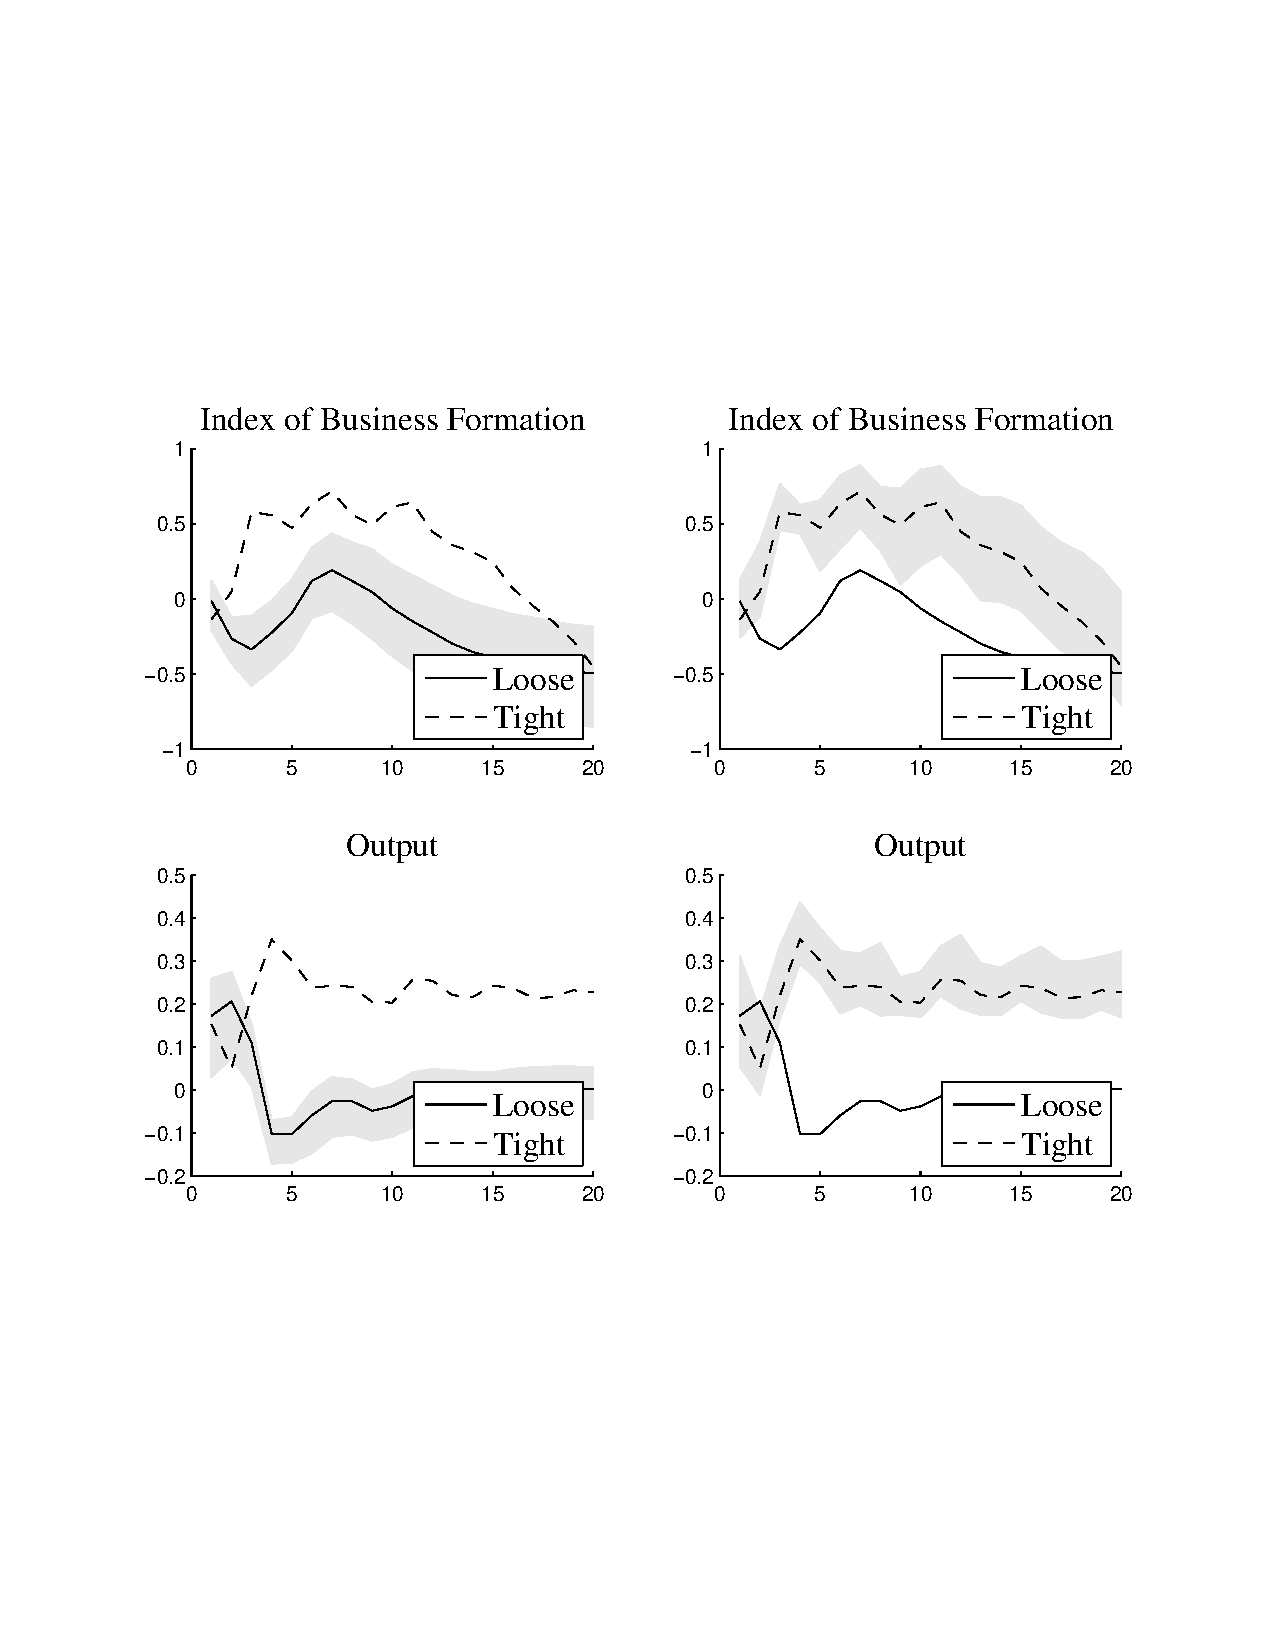
\includegraphics[trim=1cm 6.5cm 1cm 6.5cm, clip=true, width=0.9\textwidth]{graph/GShockResStateData.pdf}
\end{figure}
\end{frame}

\begin{frame}{Conclusions}
Facts:
\begin{itemize}
\item Government spending crowds out overall investment but crowds in entrepreneur activity of both entry and investment.
\item The effect is larger when credit condition is worse.
\end{itemize}
Mechanism:
\begin{itemize}
\item Entrepreneur sector uses more labor than capital due to financial frictions.
\item Change in factor prices caused by G shock increases profits of entrepreneur activity, encourages entry and investment.
\end{itemize}
Implications:
\begin{itemize}
\item An output multiplier close to data.
\item State dependence consistent with data.
\end{itemize}
\end{frame}

\begin{comment}
\begin{frame}{Entrepreneur multiplier}
\begin{figure}[!ht]
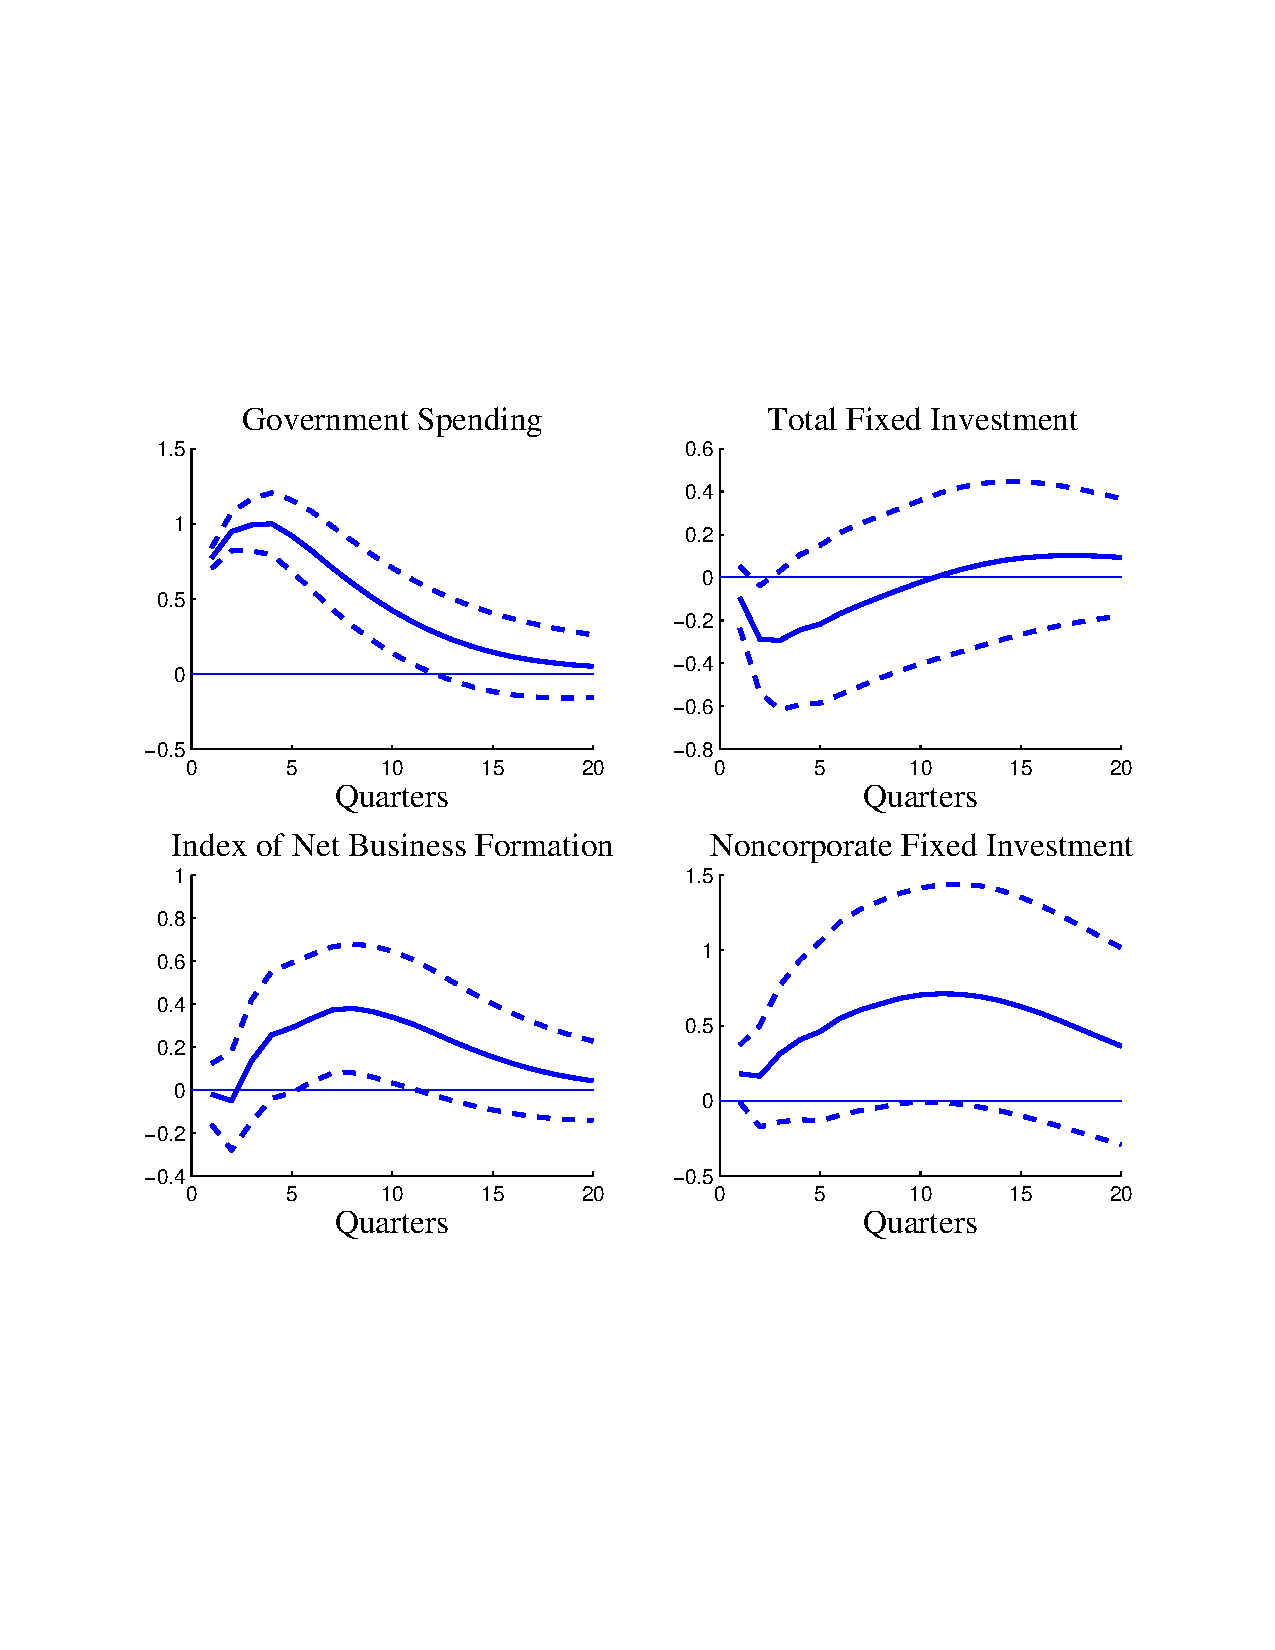
\includegraphics[trim=1cm 6.5cm 1cm 6.5cm, clip=true, width=0.9\textwidth]{graph/entre.pdf}
\end{figure}
\end{frame}

\begin{frame}{Entrepreneur multiplier: Ramey}
\begin{figure}[!ht]
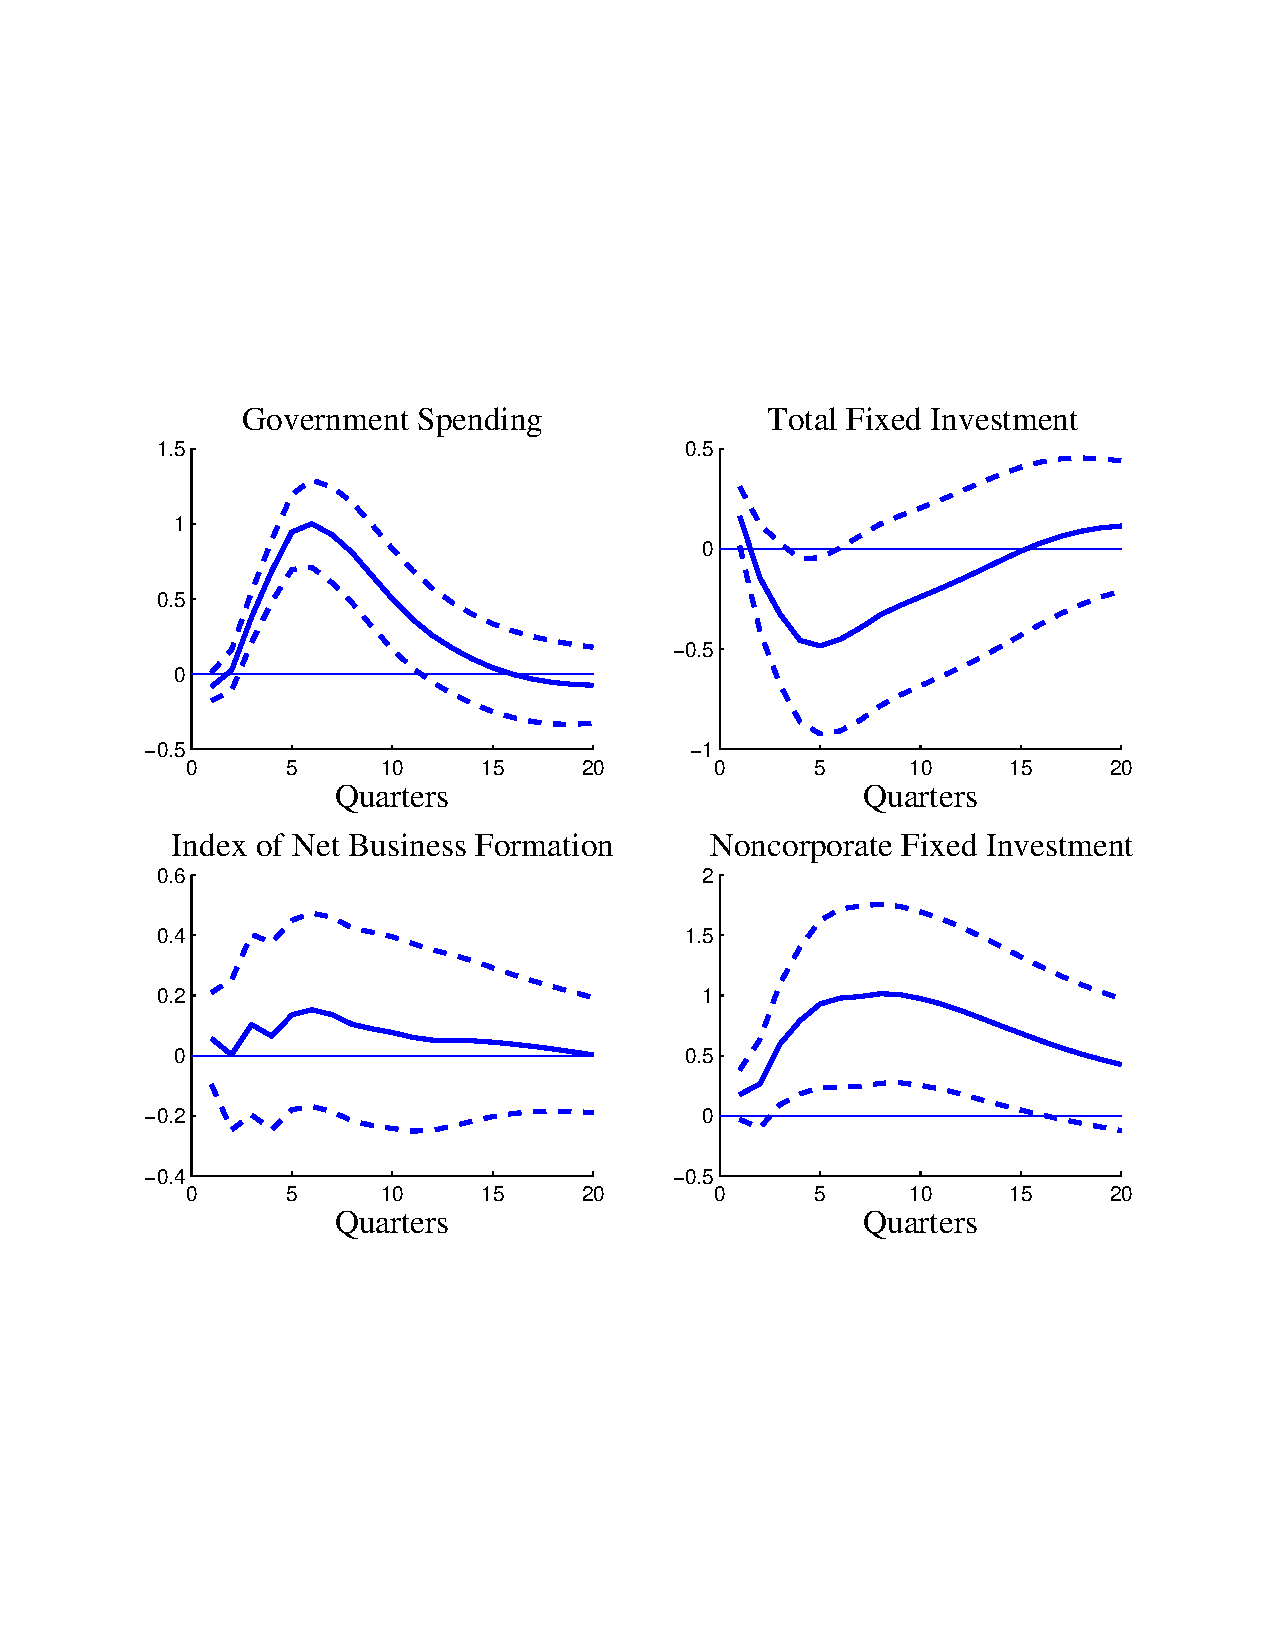
\includegraphics[trim=1cm 6.5cm 1cm 6.5cm, clip=true, width=0.9\textwidth]{graph/entre_ramey.pdf}
\end{figure}
\end{frame}

\begin{frame}{Measure of credit tightness}
Following \citet{lown_credit_2006}:
\begin{figure}%
    \centering
    \subfloat[NFCI Credit Subindex]{{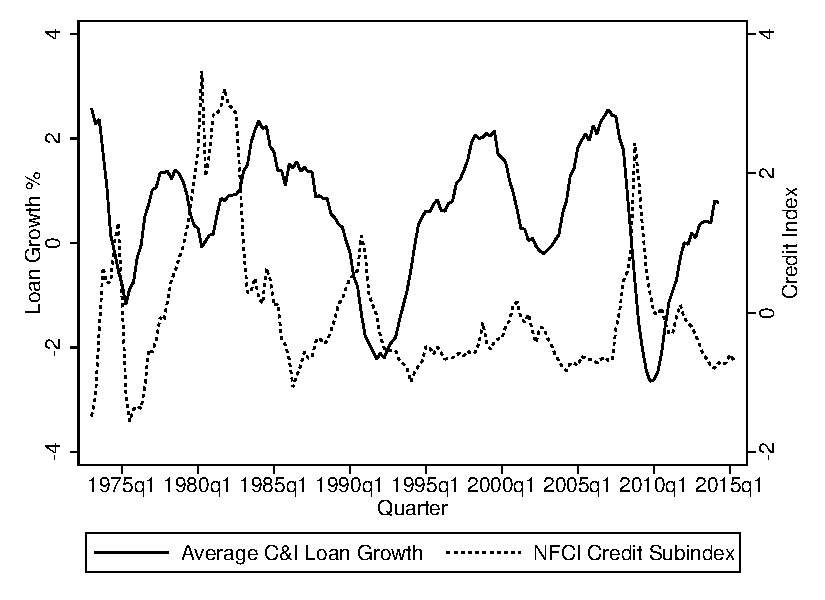
\includegraphics[width=5cm]{graph/loan_credit.pdf} }}%
    \qquad
    \subfloat[Standards: Net \% Tightning]{{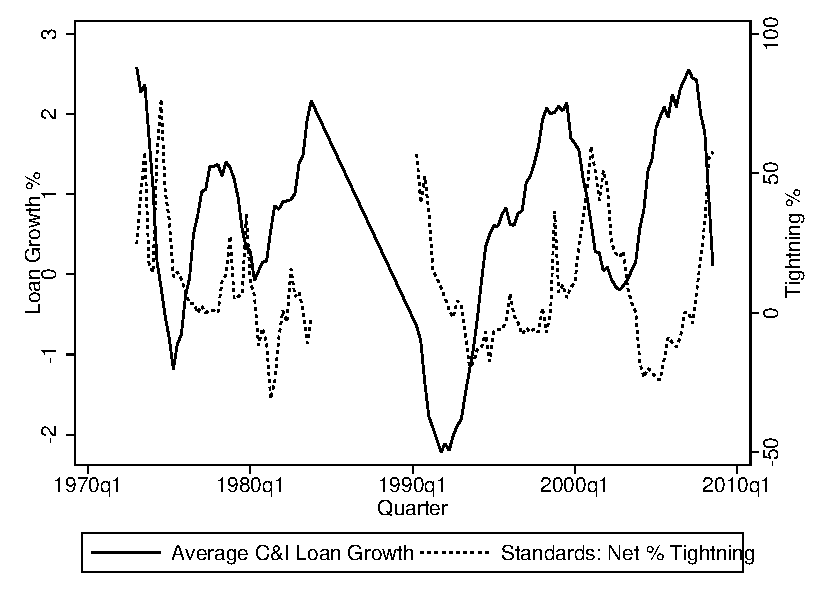
\includegraphics[width=5cm]{graph/loan_tightning.pdf} }}%
    \caption{2 C\&I Loan Growth Compared to Other Measures of Credit Tightness}%
    \label{fig:example}%
\end{figure}
\end{frame}

\begin{frame}{STVAR and state-dependent response}
Following \citet{auerbach_measuring_2012}:
\begin{figure}[!ht]
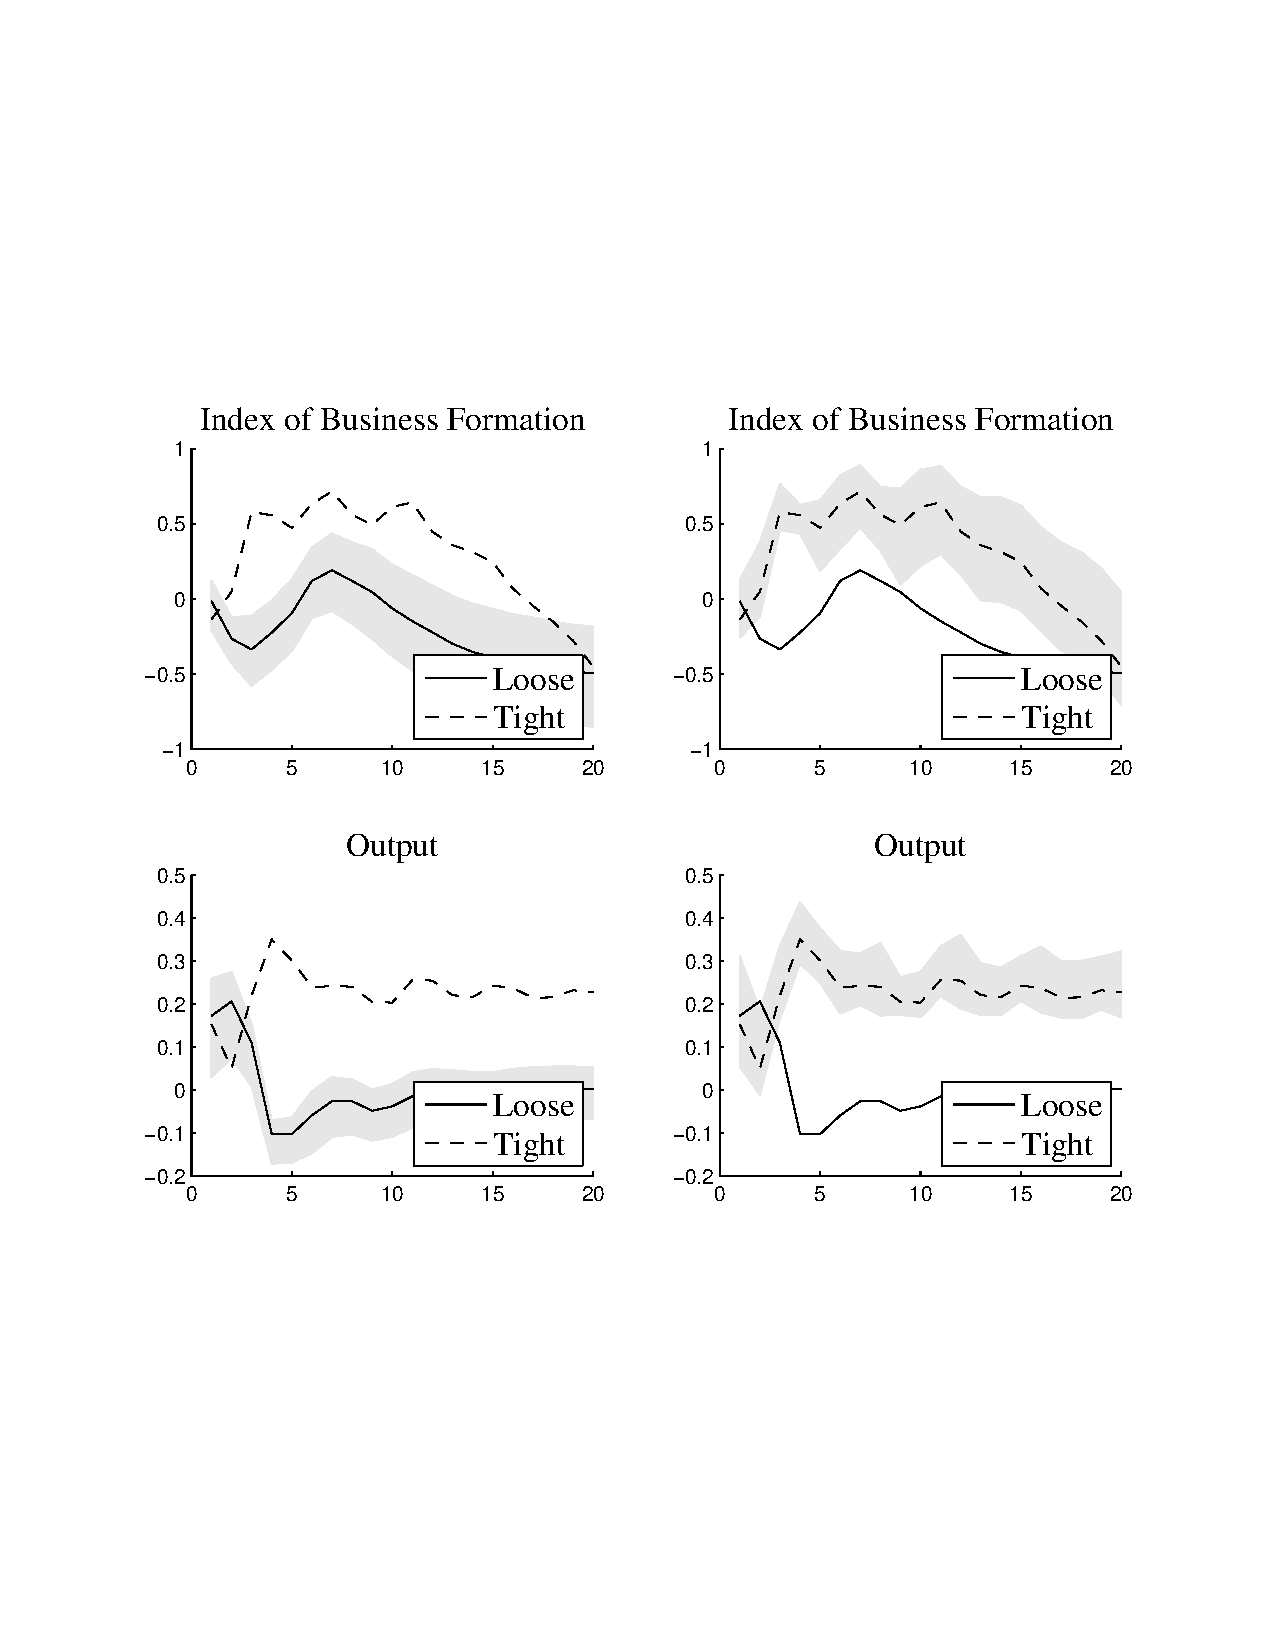
\includegraphics[trim=1cm 6.5cm 1cm 6.5cm, clip=true, width=0.9\textwidth]{graph/GShockResStateData.pdf}
\end{figure}
\end{frame}

\begin{frame}{Mechanism: credit tightness and entrepreneur factor share}
\begin{figure}%
    \centering
    \subfloat[Noncorporate Factor Share]{{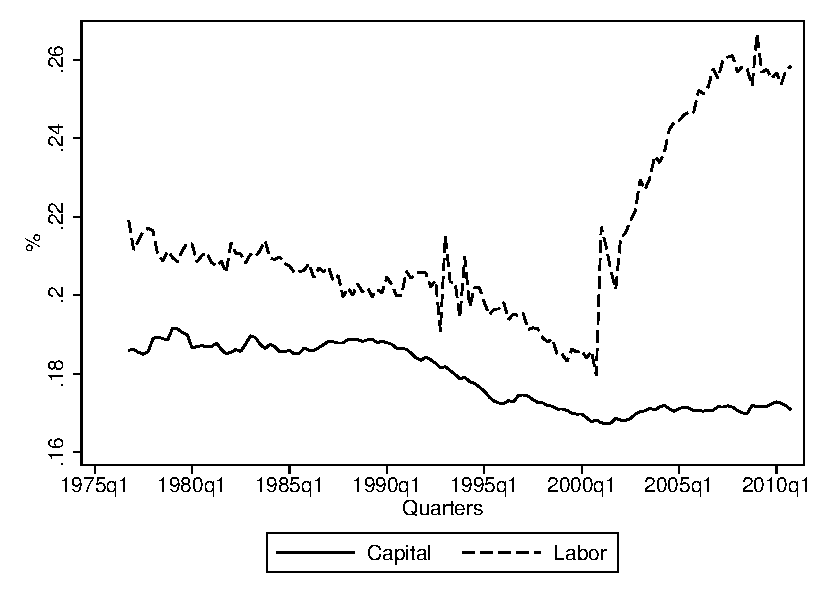
\includegraphics[width=5cm]{graph/klratio.pdf} }}%
    \qquad
    \subfloat[Tightness v.s. Factor Share]{{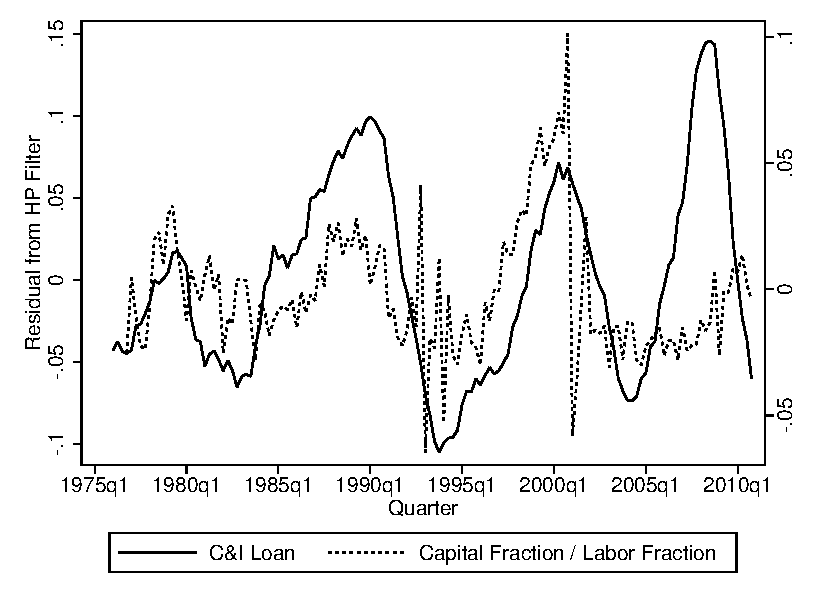
\includegraphics[width=5cm]{graph/loan_klratio.pdf} }}%
    \caption{Capital share is lower when credit is tighter}%
    \label{fig:example}%
\end{figure}
\end{frame}

\begin{frame}{Model}
\begin{itemize}
\item Occupation choice model: Quadrini (2000), Cagetti and De Nardi (2006), \citet{buera_finance_2011}
\item Augmented with endogenous labor supply and aggregate shocks (TFP, credit, and government spending shocks)
\item Government spending is unproductive, financed using debt and tax. Bachmann et al. (2015)
\item Mechanism:
\begin{itemize}
\item Government spending shock encourages labor supply through wealth effects, lowers wages, and drives up interest rates.
\item Entrepreneurs face credit constraints, which implies (1) profit and production scale are constrained by the {\bf quantity} of capital, and the {\bf price} of labor; (2) capital labor ratio is lower than corporate sector.
\item Lower wage and higher interest rate increase profit, and therefore encourages entry. Effects are larger when credit is tighter because capital labor share is even lower.
\item Future production scale increases, return to saving increases, encourages entrepreneur saving.
\end{itemize}
\end{itemize}
\end{frame}

\begin{frame}{Household's problem}
Individual states: $x=(\varepsilon,\zeta,a)$, aggregate states: $\Pi=(z,\lambda,G,B,\Phi)$
$$
V(x,\Pi)=E_{\eta}[\max \{V^W(x,\Pi),V^E(x,\Pi)+\eta\}]
$$
Worker:
$$
V^W(x,\Pi)=\max_{c,n,a'}u(c,n)+\beta EV(x',\Pi')
$$
s.t.
$$
\begin{aligned}
& c+a' \leq a(1+r(\Pi)) + w(\Pi)\varepsilon n - Tax(\Pi)\\
& a'\geq 0,0\leq n\leq 1
\end{aligned}
$$
\end{frame}

\begin{frame}{Household's problem}
Individual states: $x=(\varepsilon,\zeta,a)$, aggregate states: $\Pi=(z,\lambda,G,B,\Phi)$
$$
V(x,\Pi)=E_{\eta}[\max \{V^W(x,\Pi),V^E(x,\Pi)+\eta\}]
$$
Entrepreneur:
$$
V^E(x,\Pi)=\max_{c,n,a',k_E,n_E}u(c,n)+\beta EV(x',\Pi')
$$
s.t.
$$
\begin{aligned}
& c+a' \leq \pi\\
& \pi= z \zeta (k_E^{\gamma}(n_E+\varepsilon n)^{1-\gamma})^{\theta} + (1-\delta)k_E - (1+r(\Pi))(k_E-a) \\
& \quad \quad - w(\Pi)n_E - Tax(\Pi)\\
& k_E \leq (1+\lambda)a \\
& a'\geq 0,0\leq n\leq 1
\end{aligned}
$$
\end{frame}

\begin{frame}{Government's budget (transition rule of B')}
Bachmann et al. (2015). Key assumption: state-contingent return of government bond.
$$
\frac{Tax(\Pi)}{Y(\Pi)} = \rho_0 + \rho_1*\frac{B}{Y(\Pi)} +\rho_2*\frac{G}{Y(\Pi)}
$$
$$
B'(\Pi) = (1+r(\Pi))*B + G - Tax(\Pi)
$$
\end{frame}

\begin{frame}{Definition of recursive equilibrium}
A recursive equilibrium is: value function $\{V(x,\Pi), V^W(x,\Pi), V^E(x,\Pi)\}$, policy function $\{a'(x,\Pi),n(x,\Pi),k_E(x,\Pi),n_E(x,\Pi),\mathbf{1}^E(x,\Pi)\}$, prices and taxes $\{r(\Pi),w(\Pi),Tax(\Pi)\}$, transition of distribution $\Phi' = H(\Pi)$
\begin{itemize}
\item $r(\Pi)=\gamma z(\frac{K_C(\Pi)}{L_C(\Pi)})^{\gamma-1}-\delta$;
$w(\Pi)=(1-\gamma) z(\frac{K_C(\Pi)}{L_C(\Pi)})^\gamma$
\item $\int k_E(x,\Pi) \ d\Phi(x) + K_C(\Pi) + B = \int a(x,\Pi) \ d\Phi(x)$
\item $\int n_E(x,\Pi) \ d\Phi(x) + L_C(\Pi) = \int n(x,\Pi)(1-\mathbf{1}^E(x,\Pi)) \ d\Phi(x)$
\item Transition of B' described before
\item Transition of $\Phi$ consistent.
\end{itemize}
\end{frame}

\begin{frame}{Partial equilibrium analytical results}
Assume $n=0$ for entrepreneurs. Fix aggregate states $\Pi$,

Denote entrepreneur profit
$\pi(x;K_C,L_C,\lambda)= \max_{k_E,n_E} z \zeta (k_E^{\gamma}n_E^{1-\gamma})^{\theta} - (r+\delta)k_E- wn_E$, s.t. $k_E \leq (1+\lambda)a$

$r=\gamma z(\frac{K_C}{L_C})^{\gamma-1}-\delta$, $w=(1-\gamma) z(\frac{K_C}{L_C})^\gamma$
\begin{proposition}
$\forall s=(x,K_C,L_C)$, $\exists \bar{\lambda}(s)$, s.t.
\begin{enumerate}
\item $\forall \lambda \geq \bar{\lambda}(s)$, $\frac{k_E(s,\lambda)}{n_E(s,\lambda)}=\frac{K_C}{L_C}$
\item $\forall \lambda < \bar{\lambda}(s)$, $\frac{k_E(s,\lambda)}{n_E(s,\lambda)}<\frac{K_C}{L_C}$ and is strictly increasing in $\lambda$
\item $\forall \lambda \geq \bar{\lambda}(s)$, $\frac{\partial \pi(s,\lambda)}{\partial L_C}=0$
\item $\forall \lambda < \bar{\lambda}(s)$, $\frac{\partial \pi(s,\lambda)}{\partial L_C}>0$
\end{enumerate}
\end{proposition}
\end{frame}

\begin{frame}{Full model solution}
Following \citet{krusell_income_1998}, track $\Phi$ using $\bar{K}$. $\Phi = (z,G,\bar{K},B)$.

Approximate transition rule using polynomials of $(\bar{K},B)$.

$$
\begin{aligned}
log(\bar{K'}) = b_{1,0}(z,G,\lambda) + b_{1,1}log(\bar{K}) + b_{1,2}B + b_{1,3}B^2 + b_{1,4}B^3 \\ 
log(r+\delta) = b_{2,0} + b_{2,1}log(\bar{K}) + b_{2,2}B + b_{2,3}B^2 + b_{1,4}B^3 \\ 
log(w) = b_{3,0} + b_{3,1}log(\bar{K}) + b_{3,2}B + b_{3,3}B^2 + b_{3,4}B^3 \\ 
log(Tr) = b_{4,0} + b_{4,1}log(\bar{K}) + b_{4,2}B + b_{4,3}B^2 + b_{4,4}B^3 \\ 
\end{aligned}
$$
\end{frame}

\begin{frame}{Calibration: parameters fixed exogenously}
$u=\frac{c^{1-\sigma}}{1-\sigma}-\chi \frac{n^{1+1/ \nu}}{1+1 / \nu}$, $\sigma=2$, $\nu=0.5$

$F(K_C,L_C) = zK_C^{\gamma}L_C^{1-\gamma}$, $\gamma=0.33$

$\varepsilon$, $\varepsilon'=\rho_{\varepsilon}\varepsilon + e'$, $\rho_{\varepsilon}=0.94$,$\sigma^2_{\varepsilon}=0.01$

$z$, $\rho_z=0.9$, $\sigma_z=0.01$

$G$, Bachmann et al. (2015)

$\eta$, Gumbel distribution with scale parameter 1
\end{frame}

\begin{frame}{Calibration: parameters calibrated to match moments}
\begin{table}[htbp]
  \centering
    \begin{tabular}{ccccc}
    \toprule
    Parameters & Value & Target & Data  & Model \\
    \midrule
    $\delta$ & 0.0157 & r     & 0.0125 & 0.0125 \\
    $\beta$ & 0.9768 & K/Y &  10.6 & 10.51 \\
    $\chi$ & 51.0788  & $\bar{n_w}$ & 0.33  & 0.33 \\
    \midrule
    $p_1$ & 0.0023  & \% Entrepreneurs & 0.0755  & 0.0755 \\
    $p_2$ & 0.9808 & Gini & 0.81 & 0.80 \\
    $\mu_{\zeta}$ & 0.4172     & \% Size 1-5 & 0.7568 & 0.7510 \\
    $\sigma_{\zeta}$ & 0.3843 & \% Size 6-10 & 0.1124 & 0.1460 \\
    \midrule
    $\theta$ & 0.7131 & Capital share & 0.1780 & 0.1779 \\
    $\lambda$ & 1.1481 & Labor share & 0.2180  & 0.2189 \\
    \midrule
    $Tax$ & 0.2497 & G/Y & 0.2086 & 0.2080 \\
    Government Bond & 0.3597 & B/Y & 0.3000 & 0.2996 \\
    \bottomrule
    \end{tabular}%
  \label{tab:addlabel}%
\end{table}%
\end{frame}

\begin{frame}{Calibration: size and wealth distribution}
Size of entrepreneur firms measured by employment level, KFS
\begin{table}[htbp]
  \centering
  
    \begin{tabular}{cccccc}
    \toprule
    & 1-4 & 5-9 & 10-19 & 20-99 & 100+ \\
    Data & 75.1 & 14.6 &  6.6  & 3.5  & 0.3 \\
    Model & 75.6 & 11.2 & 6.5 & 6.2 & 0.2 \\
    \bottomrule
    \end{tabular}%
    
\end{table}
Wealth distribution, SCF, \citet{diaz-gimenez_facts_2011}
\begin{table}[htbp]
  \centering
  
    \begin{tabular}{cccccc}
    \toprule
    & Top 1\% & Top 5\% & Top 10\% & Top 20\% & Gini\\
    Data & 30 & 51 & 64 & 79 & 0.79 \\
Model & 30.2 & 62.1 & 75.5 & 86.2 & 0.80 \\
\bottomrule
    \end{tabular}%
\end{table}
\end{frame}

\begin{frame}{Entrepreneur fiscal multiplier}
\begin{figure}[!ht]
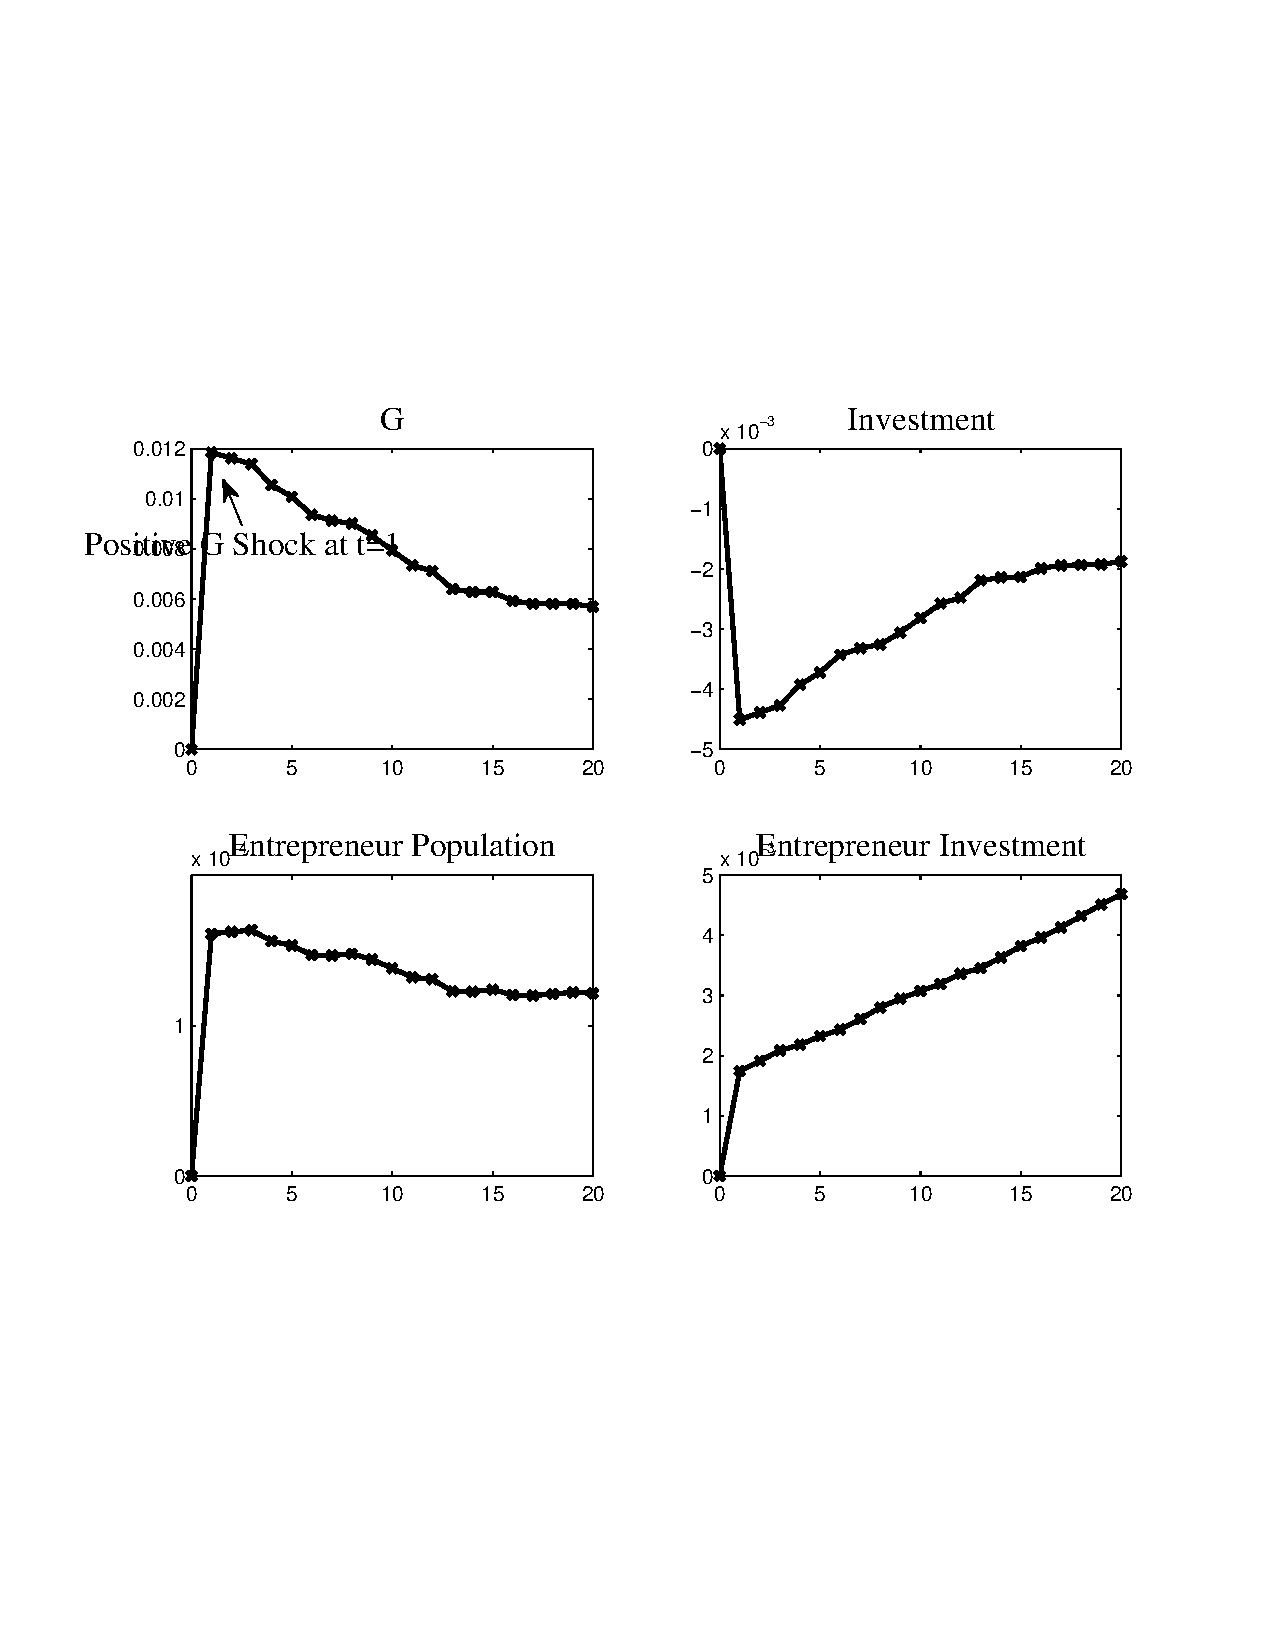
\includegraphics[trim=1cm 6.5cm 1cm 6.5cm, clip=true, width=0.9\textwidth]{graph/GShockRes.pdf}
\end{figure}
\end{frame}

\begin{frame}{Entrepreneur fiscal multiplier}
\begin{figure}[!ht]
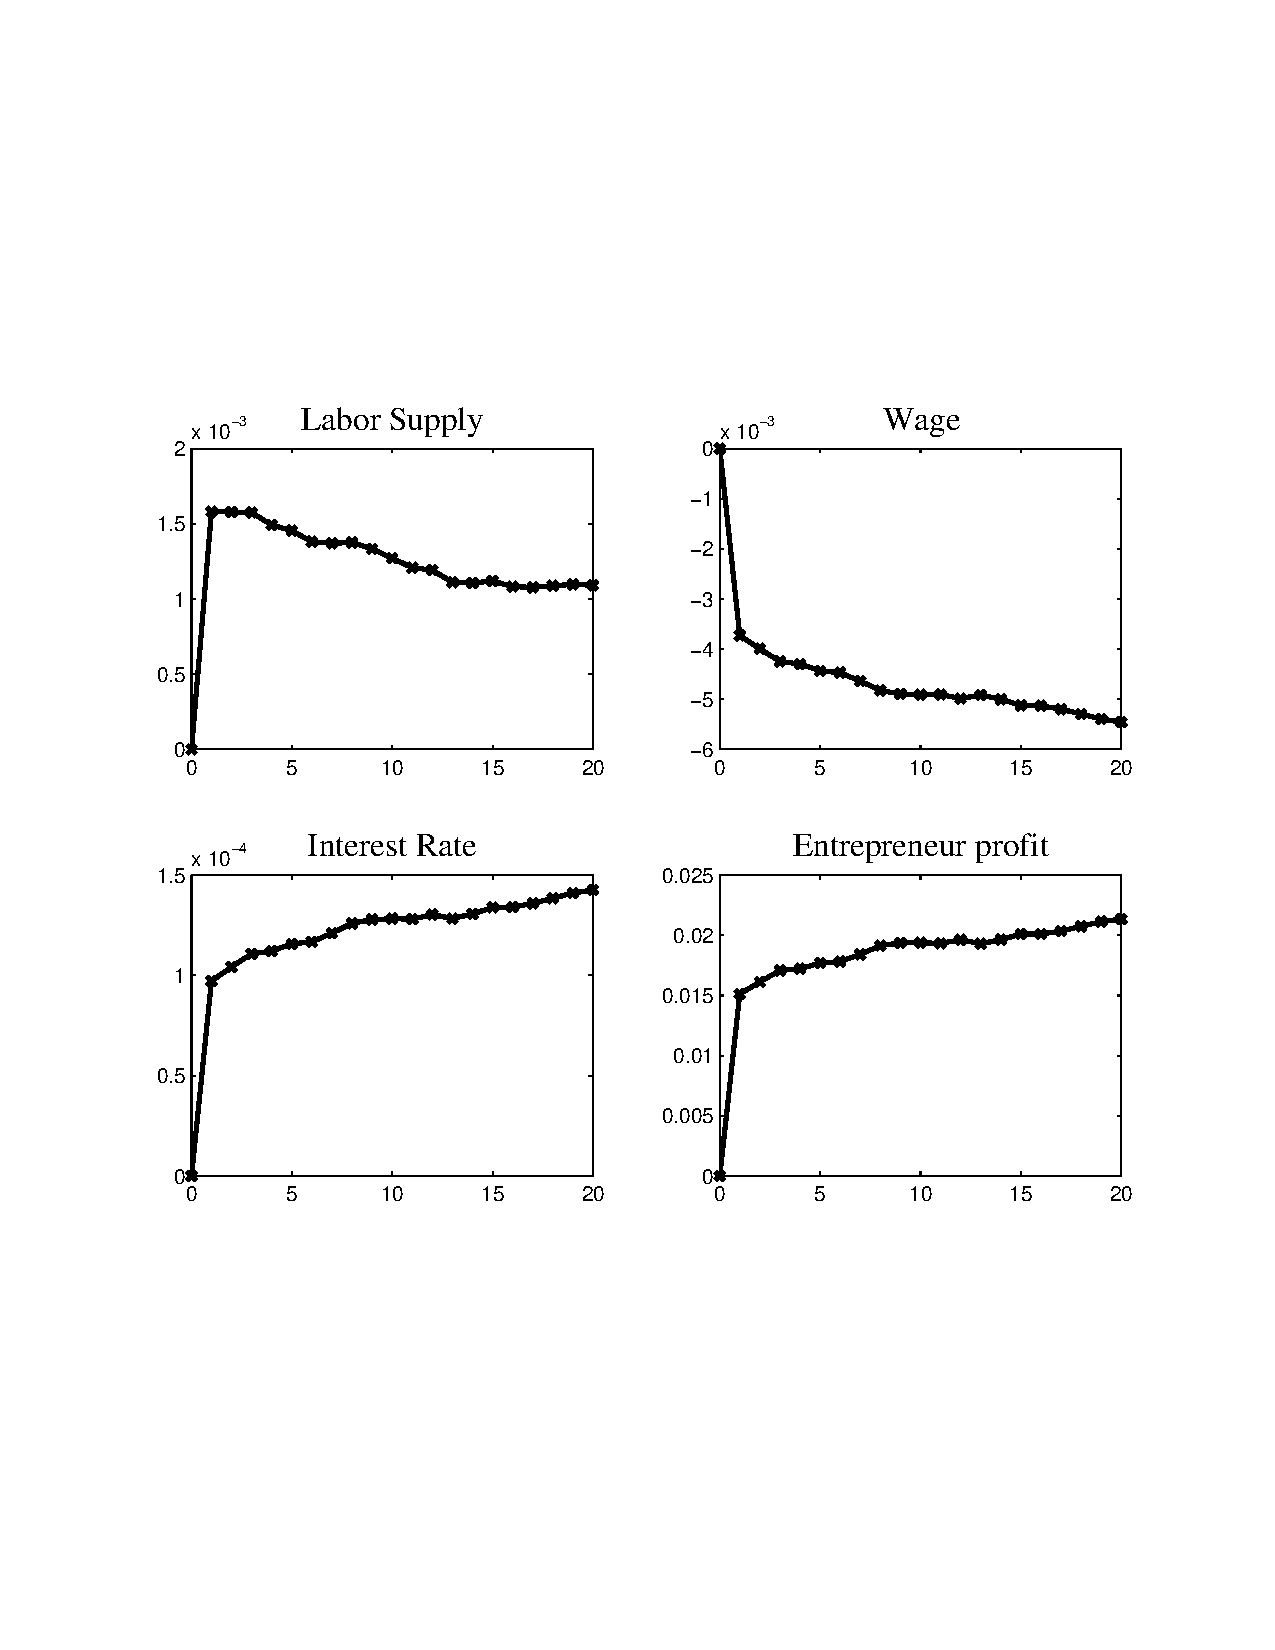
\includegraphics[trim=1cm 6.5cm 1cm 6.5cm, clip=true, width=0.9\textwidth]{graph/GShockMechanism.pdf}
\end{figure}
\end{frame}

\begin{frame}{Implied output multiplier}
\begin{figure}[!ht]
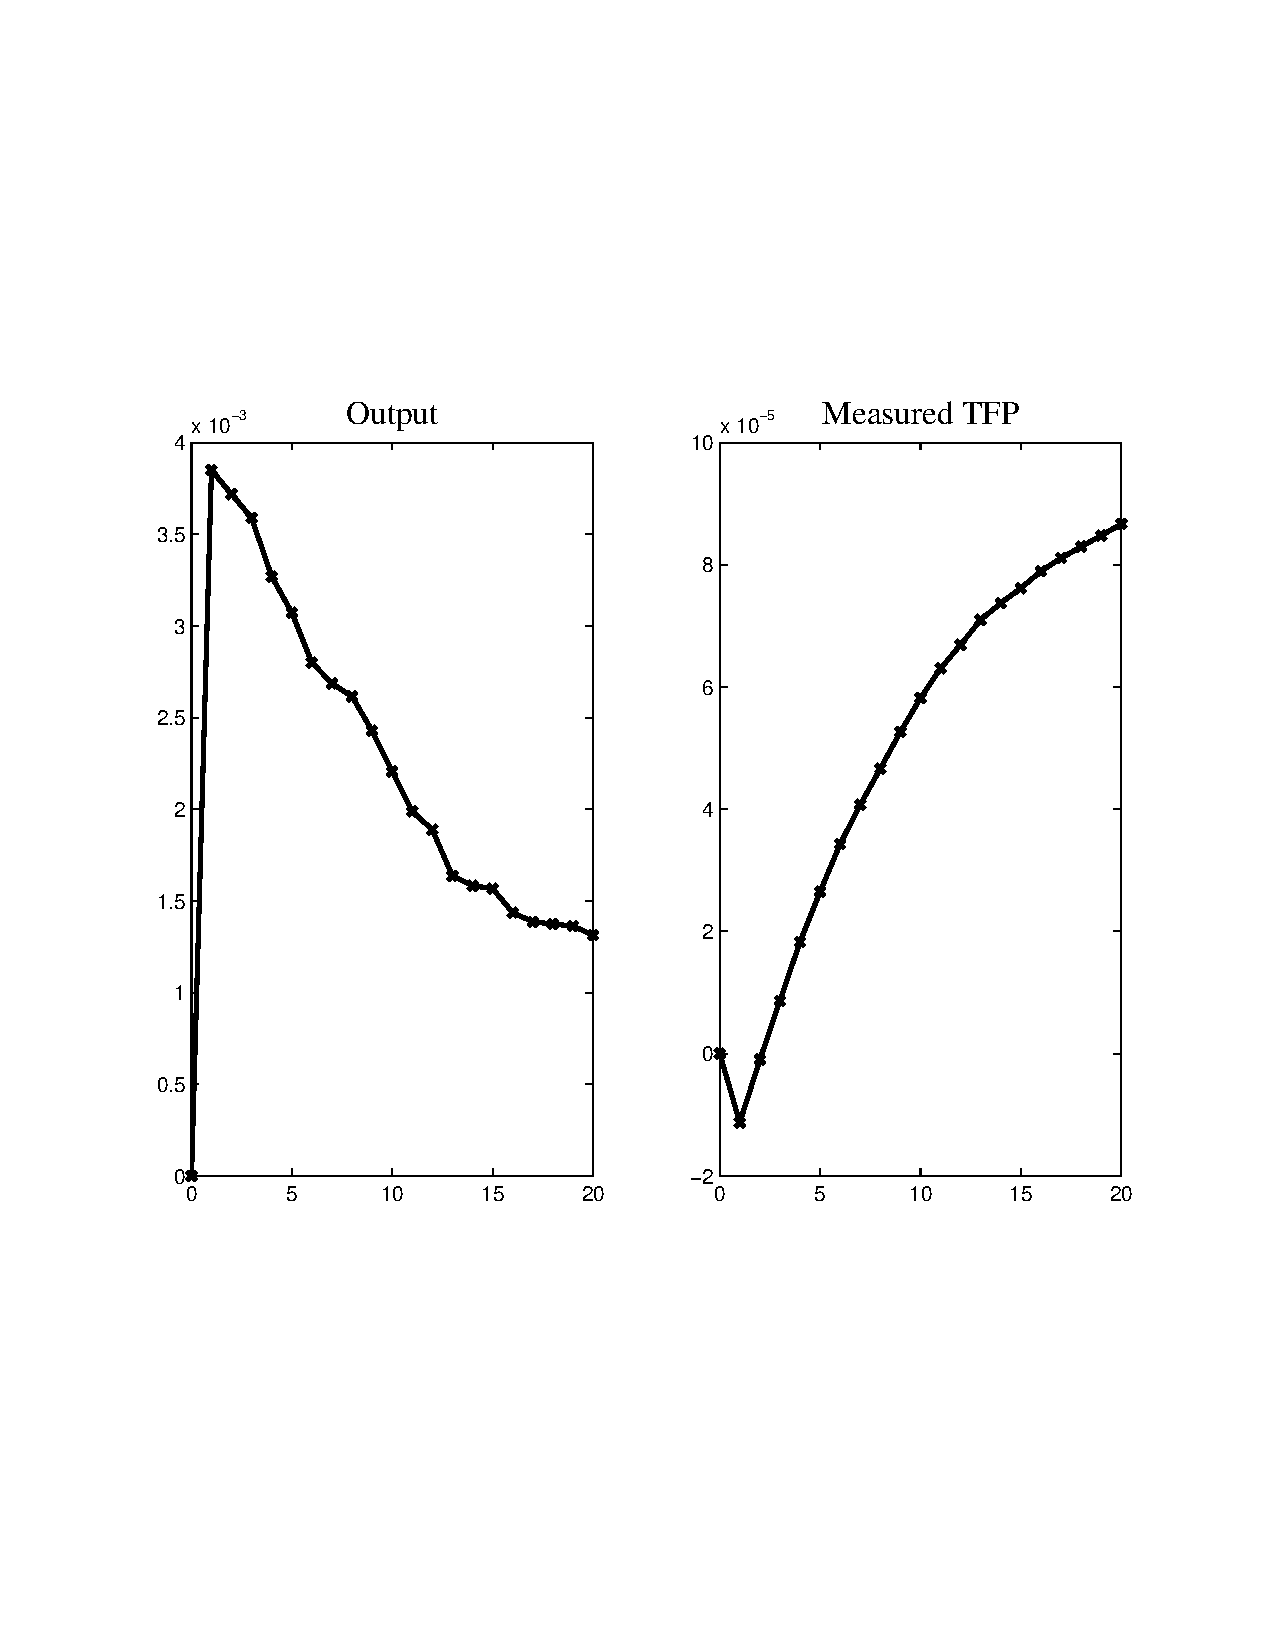
\includegraphics[trim=1cm 6.5cm 1cm 6.5cm, clip=true, width=0.9\textwidth]{graph/GShockOutput.pdf}
\end{figure}
\end{frame}

\begin{frame}{State dependence: a credit crunch}
\begin{figure}[!ht]
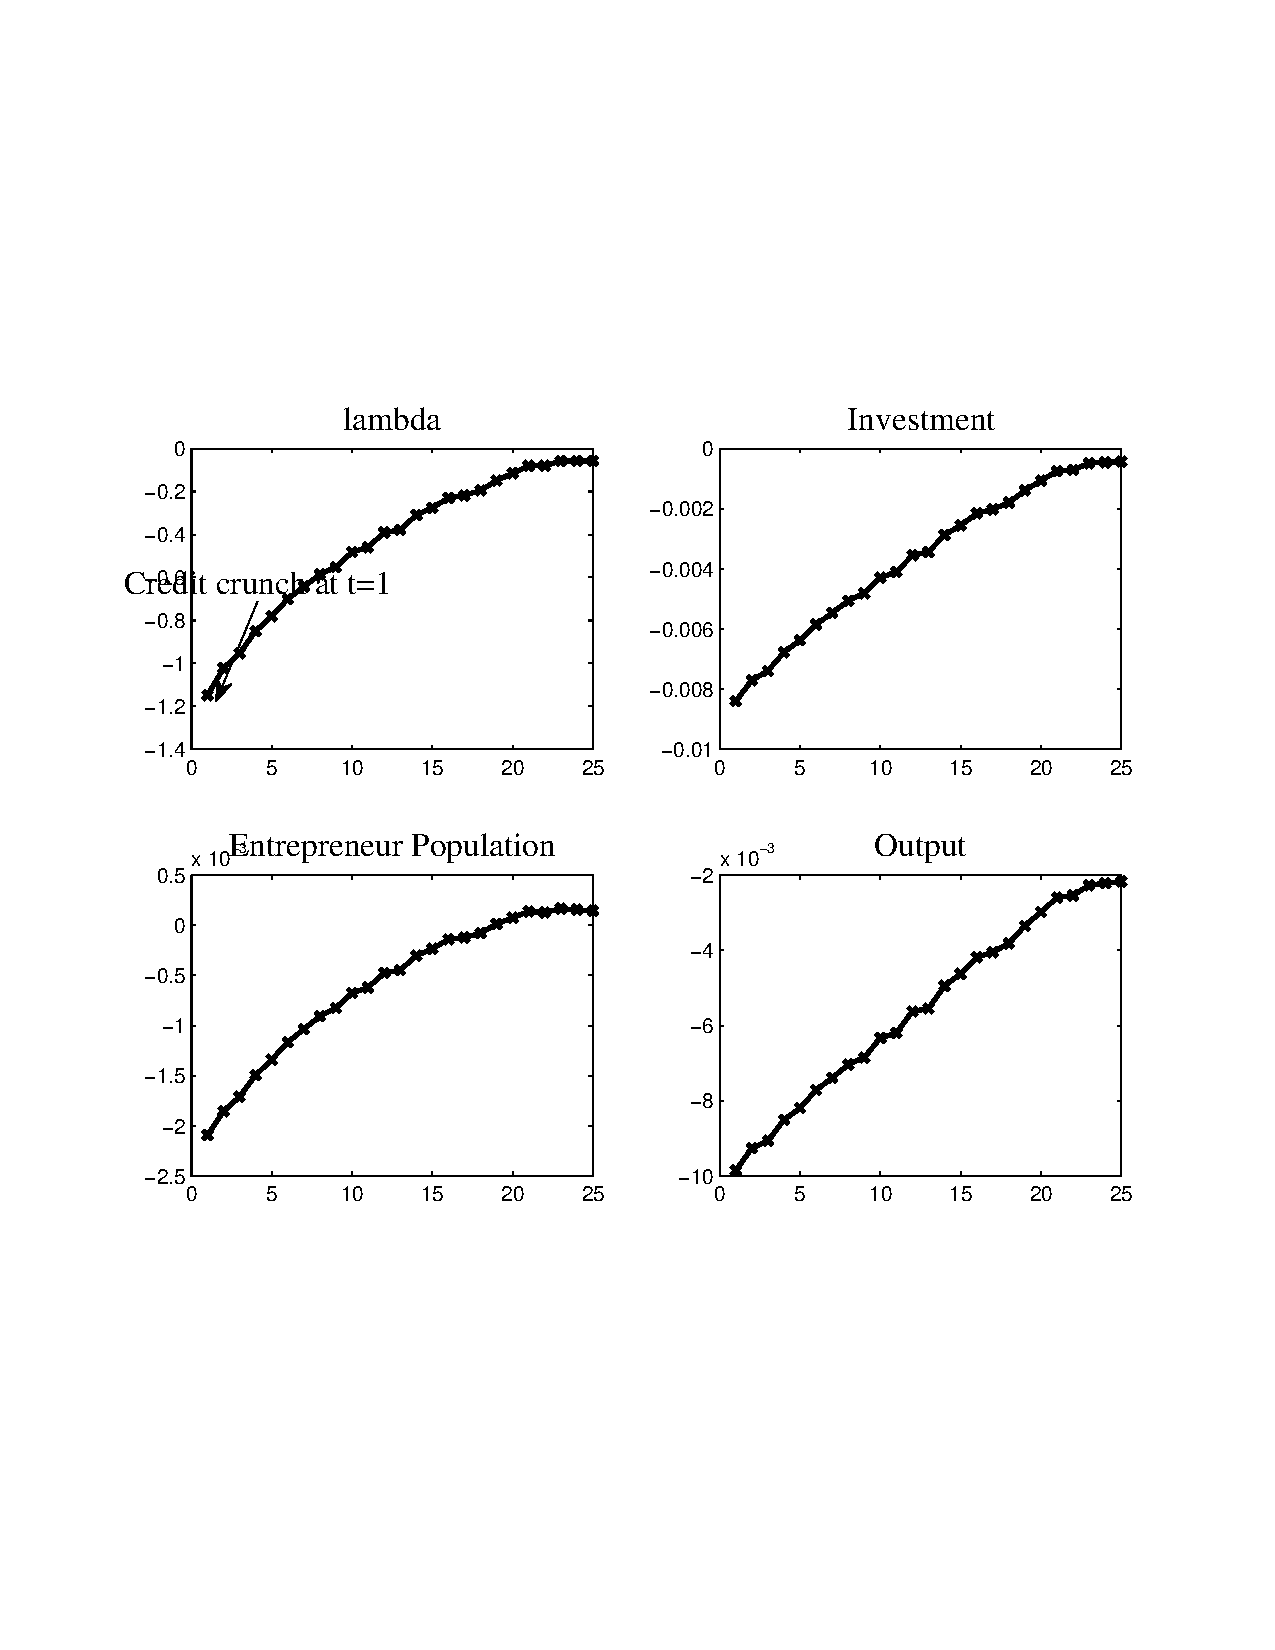
\includegraphics[trim=1cm 6.5cm 1cm 6.5cm, clip=true, width=0.9\textwidth]{graph/LambdaShockRes.pdf}
\end{figure}
\end{frame}

\begin{frame}{State dependence: fiscal multiplier at a credit crunch}
\begin{figure}[!ht]
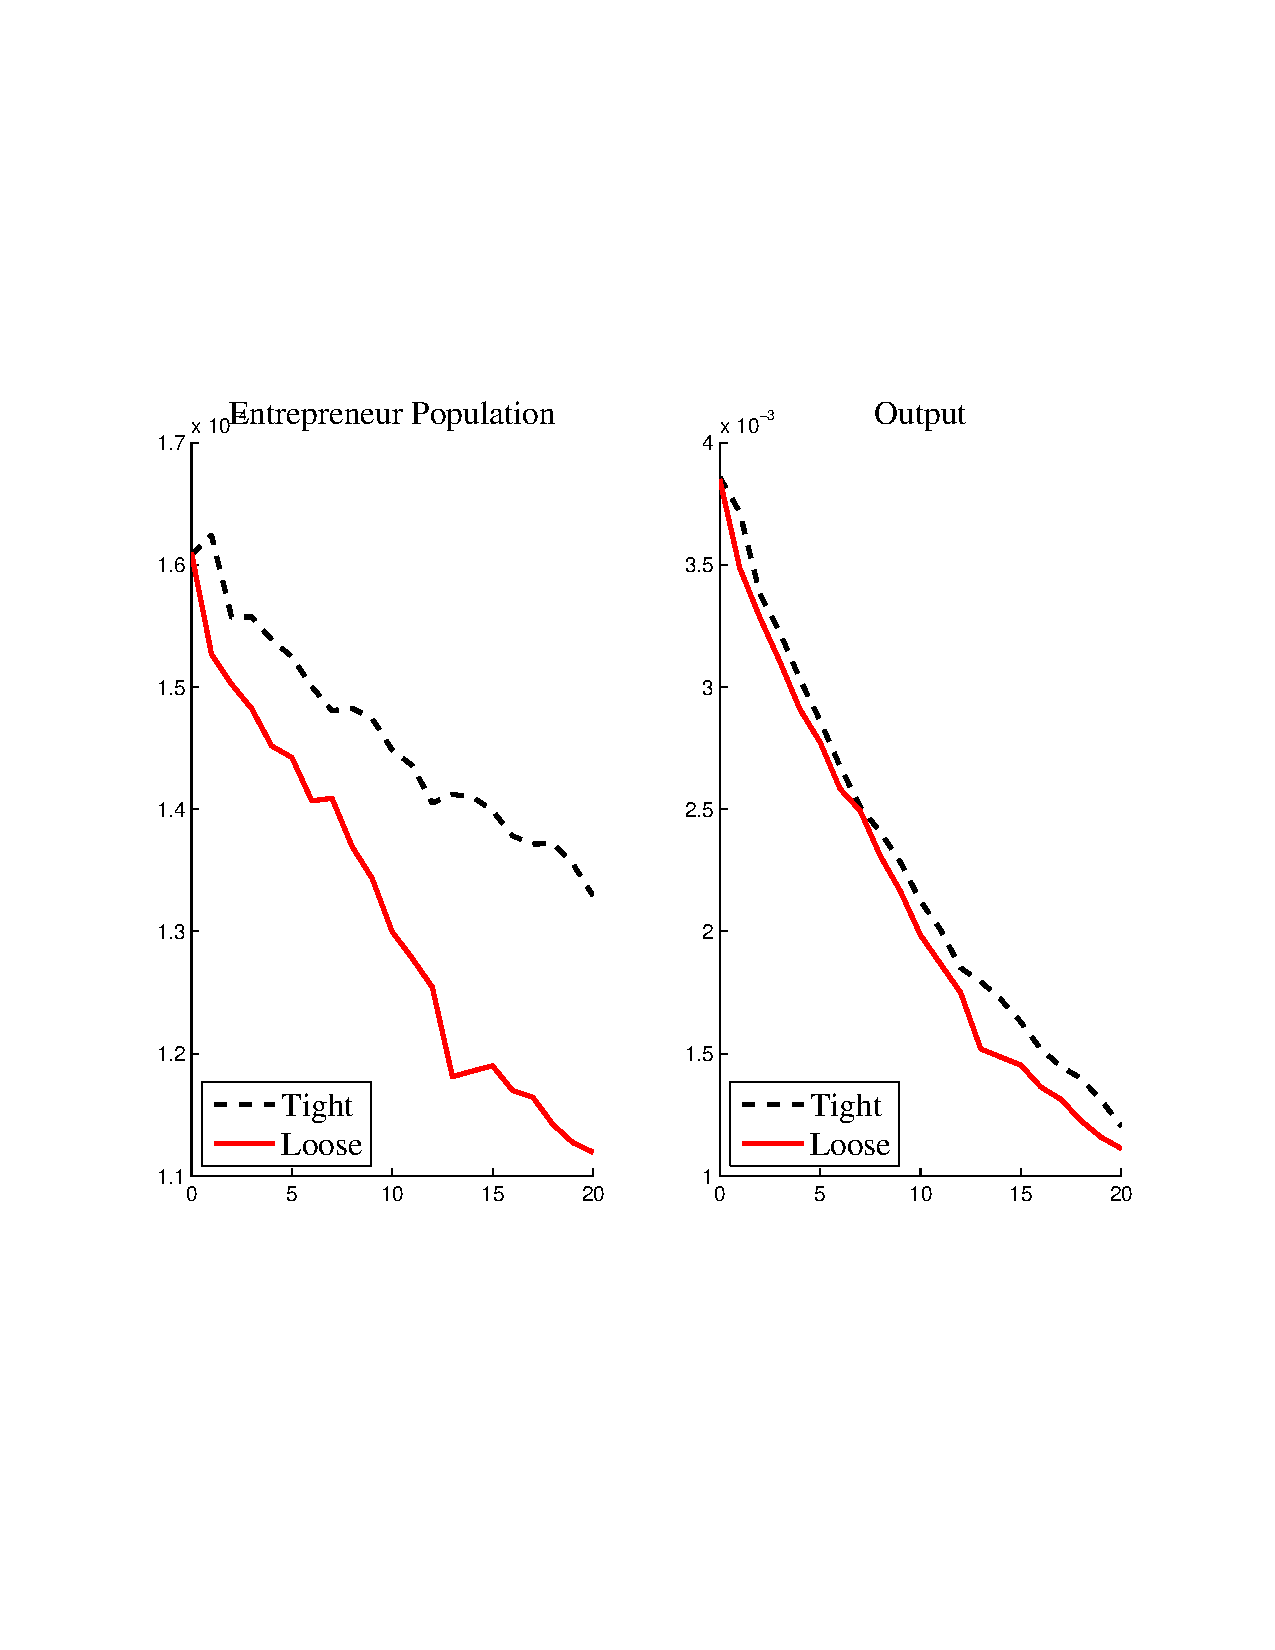
\includegraphics[trim=1cm 6.5cm 1cm 6.5cm, clip=true, width=0.9\textwidth]{graph/GShockResStateLambda.pdf}
\end{figure}
\end{frame}

\begin{frame}{Conclusions}
\begin{itemize}
\item A new transmission mechanism of government spending: increases labor supply and encourages entrepreneurship.
\item The entrepreneur multiplier and the implied output multiplier are larger when credit is tighter.
\item Effects and mechanism are consistent with data.
\end{itemize}
\end{frame}


\begin{comment}
\begin{frame}{Entrepreneur multiplier over business cycle}
\begin{figure}[!ht]
\includegraphics[clip=true, width=0.5\textwidth]{graph/formation_state.pdf}
\includegraphics[clip=true, width=0.5\textwidth]{graph/ncfi_state.pdf}
\end{figure}
\end{frame}









\begin{frame}{Solution}
KS, track $\Phi$ using $\bar{K}$. $\Phi = (z,G,\bar{K},B)$.

Approximate transition rule using polynomials of $(\bar{K},B)$.

$$
\begin{aligned}
log(\bar{K'}) = b_{1,0} + b_{1,1}log(\bar{K}) + b_{1,2}B + b_{1,3}B^2 + b_{1,4}B^3 \\ 
log(r+\delta) = b_{2,0} + b_{2,1}log(\bar{K}) + b_{2,2}B + b_{2,3}B^2 + b_{1,4}B^3 \\ 
log(w) = b_{3,0} + b_{3,1}log(\bar{K}) + b_{3,2}B + b_{3,3}B^2 + b_{3,4}B^3 \\ 
log(Tr) = b_{4,0} + b_{4,1}log(\bar{K}) + b_{4,2}B + b_{4,3}B^2 + b_{4,4}B^3 \\ 
\end{aligned}
$$
$b$ depends on discrete $(Z,G)$
\end{frame}

\begin{frame}{Solution: a typical $R^2$}
At $(iZ=1,iG=1)$

$$
\begin{aligned}
log(\bar{K'}): 0.999995 \\ 
log(r+\delta): 0.9996 \\ 
log(w): 0.9996 \\ 
log(Tr): 0.9992 \\ 
\end{aligned}
$$
\end{frame}

\begin{frame}{Calibration}
$u=\frac{c^{1-\sigma}}{1-\sigma}-\chi \frac{n^{1+1/ \nu}}{1+1 / \nu}$, $\sigma=2$, $\nu=0.5$

$\eta$, Gumbel distribution with scale parameter 1

$\gamma=0.33$, $\theta=0.85$

$\varepsilon$, $\varepsilon'=\rho_{\varepsilon}\varepsilon + e'$, $\rho_{\varepsilon}=0.9322$

$z$, $\rho_z=0.9$, $\sigma_z=0.01$, 3 states

$G$, Bachmann et al. (2015)

$\lambda=1.5$

$\zeta$: Cagetti and De Nardi (2004), $\{0,\zeta_{\mu}\}$, with transition matrix $(1-p_1,p_1;1-p_2,p_2)$
\begin{table}[htbp]
  \centering
    \begin{tabular}{ccccc}
    \toprule
    Parameters & Value & Target & Data  & Model \\
    \midrule
    $\beta$ & 0.9768 & r     & 0.0125 & 0.0125 \\
    $\chi$ & 70    & $\bar{n_w}$ & 0.33  & 0.33 \\
    $p1$ & 8.6e-04  & Entre pop rate & 0.0755  & 0.0755 \\
    $p2$ & 0.9926 & Entre/worker wealth & 8 & 8 \\
    $\mu_{\zeta}$ & 1.74     & Entre/worker income & 4 & 4 \\
    $\sigma_{\varepsilon}$ & 0.096 & Gini & 0.81 & 0.81 \\
    \bottomrule
    \end{tabular}%
  \label{tab:addlabel}%
\end{table}%
\end{frame}

\begin{frame}{A negative z shock}
\begin{figure}[!ht]
\includegraphics[trim=1cm 6.5cm 1cm 6.5cm, clip=true, width=1\textwidth]{graph/ZShockRes.pdf}
\end{figure}
\end{frame}

\begin{frame}{A positive G shock}
\begin{figure}[!ht]
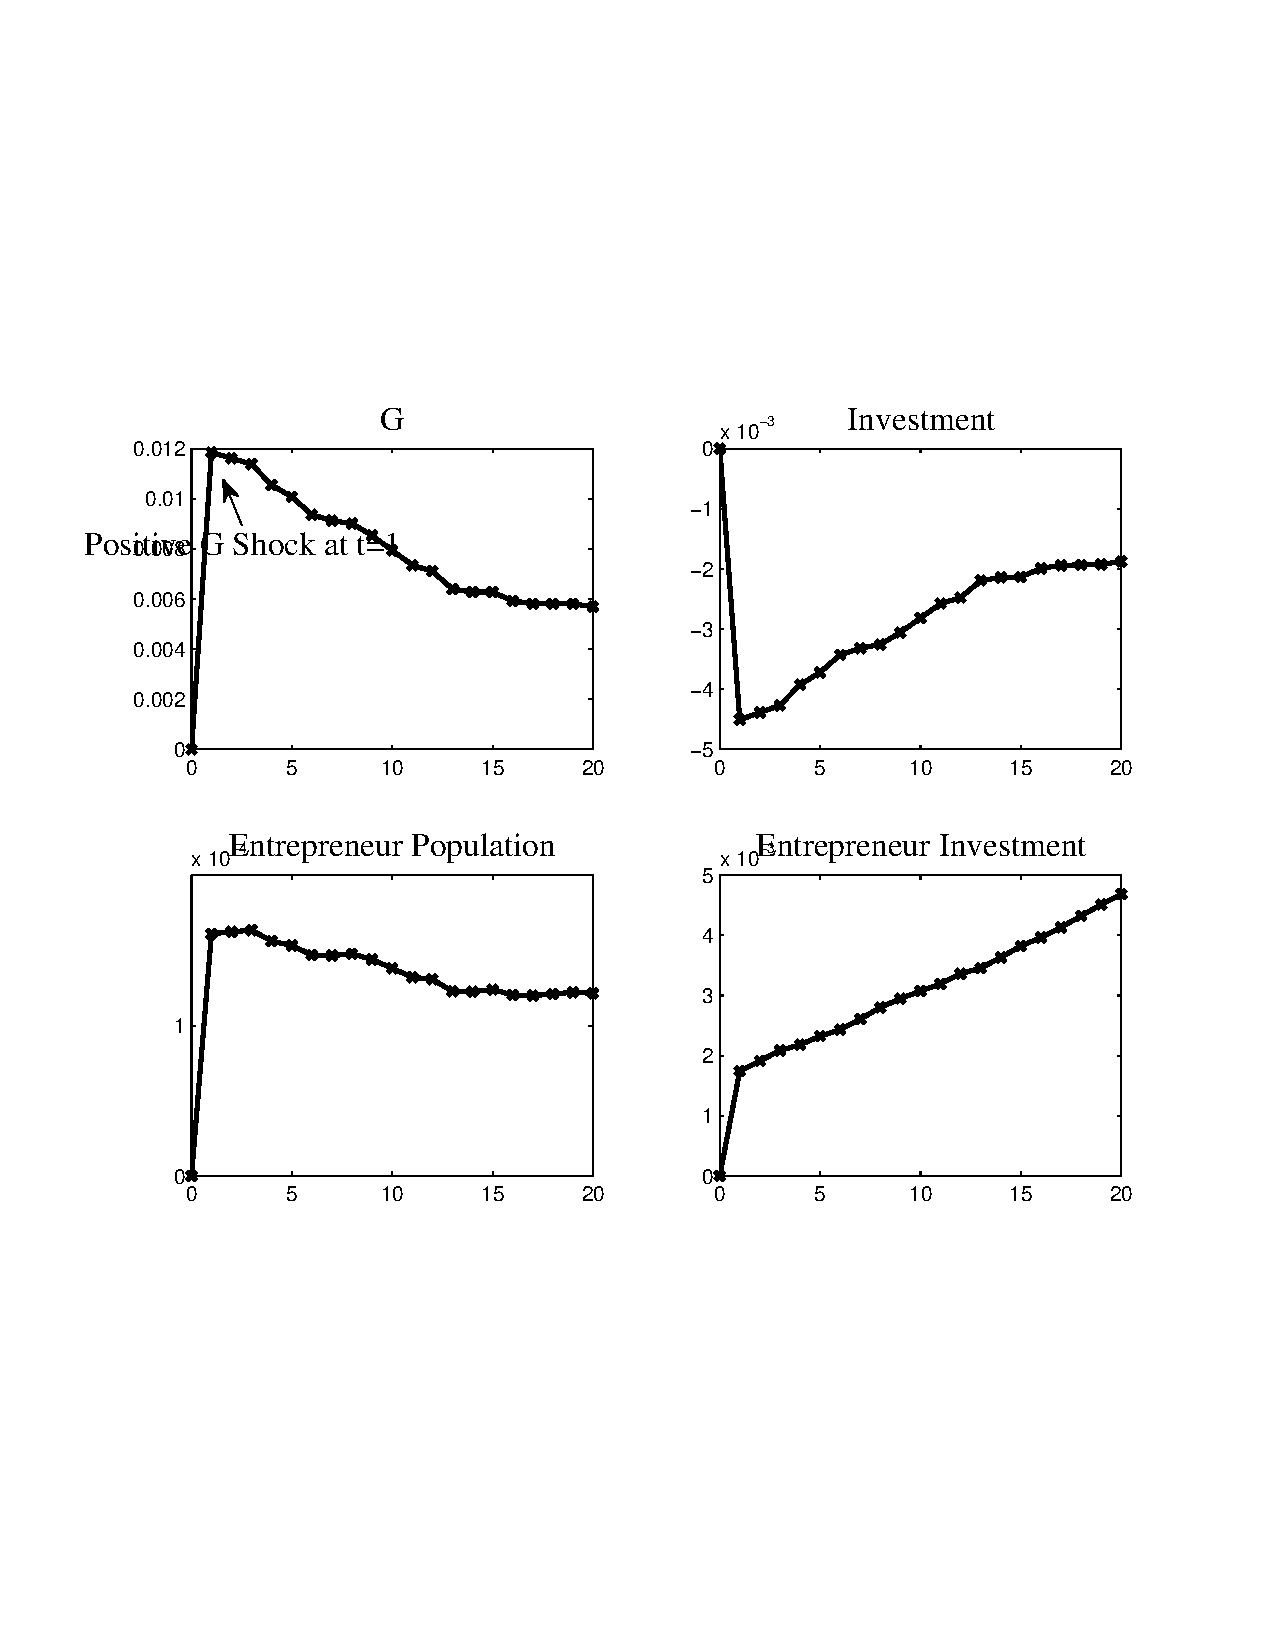
\includegraphics[trim=1cm 6.5cm 1cm 6.5cm, clip=true, width=1\textwidth]{graph/GShockRes.pdf}
\end{figure}
\end{frame}

\begin{frame}{A positive G shock in expansion and recession}
\begin{figure}[!ht]
\includegraphics[trim=1cm 6.5cm 1cm 6.5cm, clip=true, width=1\textwidth]{graph/GShockResState.pdf}
\end{figure}
\end{frame}

\begin{frame}{A positive G shock in expansion and recession}
\begin{figure}[!ht]
\caption{Index of Net Business Formation, STVAR}
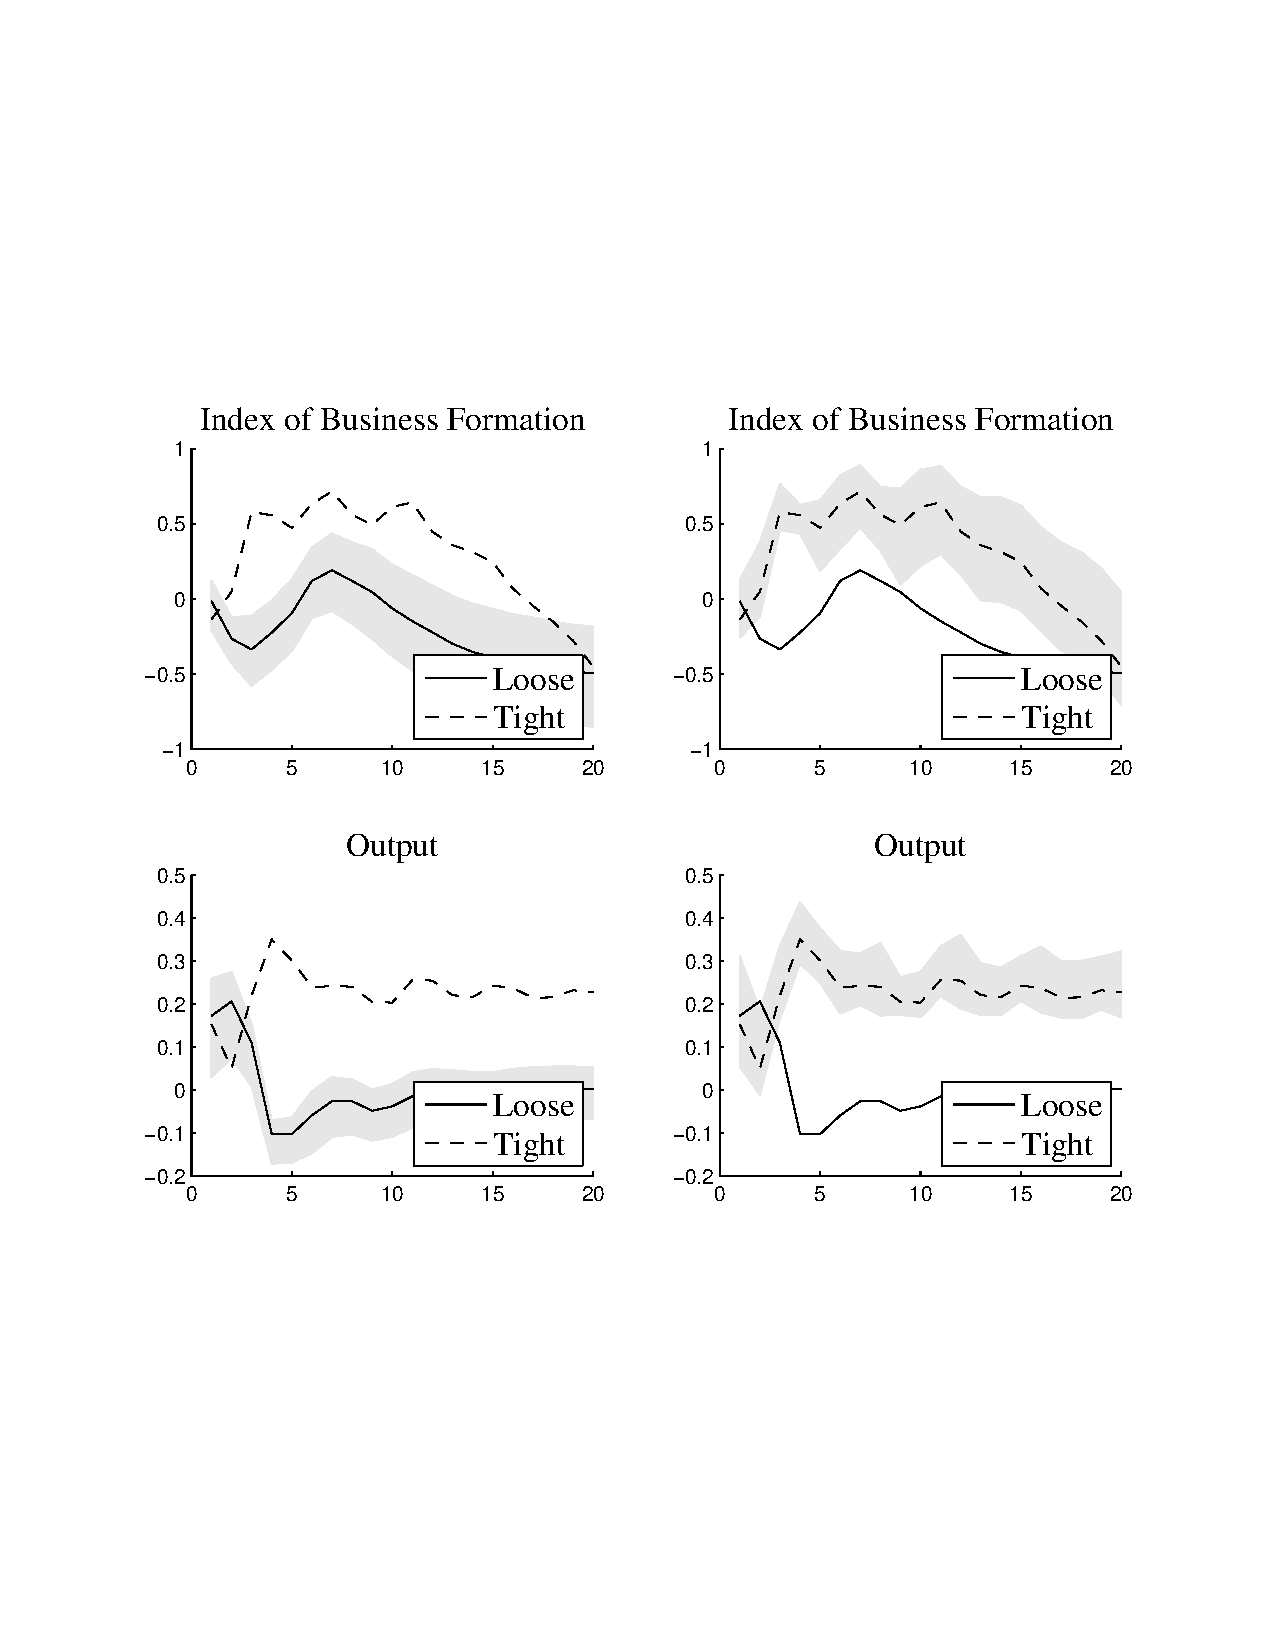
\includegraphics[trim=1cm 6.5cm 1cm 6.5cm, clip=true, width=0.8\textwidth]{graph/GShockResStateData.pdf}
\end{figure}
\end{frame}

\begin{frame}{Todo}
\begin{itemize}
\item Cross-section evidence.
\item Decompose and compare with no-entrepreneur benchmark.
\item Stylized model to show mechanism.
\item KS.
\end{itemize}
\end{frame}
\end{comment}


\bibliographystyle{economtex/aer}
\bibliography{entre}
\end{document}






